% %%%%%%%%%%%%%%%%%%%%%%%%%%%%%%%%%
% %TECH_REPORT
% \documentclass[a4paper,twoside]{article}
% %%%%%%%%%%%%%%%%%%%%%%%%%%%%%%%%%%%%%%%%
% % SPAA
% %\documentclass[11pt]{article}
% 
% \usepackage{etoolbox}
% %%%%%%%%%%%%%%%%%%%%%%%%%%%%%%%%%%%%%%%%%%%%%%%%%%%%%%%%%%%%%%%%%%%%%%%%%%%%%%
% % For deciding if this is a tech report or not
% %%%%%%%%%%%%%%%%%%%%%%%%%%%%%%%%%%%%%%%%%%%%%%%%%%%%%%%%%%%%%%%%%%%%%%%%%%%%%%
% \newtoggle{tech_report}
% \toggletrue{tech_report}
% %\togglefalse{tech_report}
% %%%%%%%%%%%%%%%%%%%%%%%%%%%%%%%%%%%%%%%%%%%%%%%%%%%%%%%%%%%%%%%%%%%%%%%%%%%%%%
% %
% %%%%%%%%%%%%%%%%%%%%%%%%%%%%%%%%%%%%%%%%%%%%%%%%%%%%%%%%%%%%%%%%%%%%%%%%%%%%%%
% 
% 
% %%%%%%%%%%%%%%%%%%%%%%%%%%%%%%%%%
% %TECH_REPORT
% \iftoggle{tech_report} {} {
% 
% % American letter size:
% \textwidth6.5in \textheight9in \oddsidemargin 0pt \evensidemargin 0pt
% \topmargin -47pt
% 
% %%%%%%%%%%%%%%%%%%%%%%%%%%%%%%%%%%%%%%%%%%%%%%%%%%%
% % endtoggle TECH_REPORT
% }
% 
% 
% 
% \usepackage{times}
% 
% \usepackage{verbatim}
% \usepackage{graphicx}
% \usepackage{amsmath,amsfonts,amssymb,latexsym}
% %\usepackage{txfonts,pxfonts,wasysym}
% \usepackage{color}
% \usepackage{flushend}
% \usepackage{subfigure}
% \usepackage{multicol}
% \usepackage{hhline}
% \usepackage{cite}
% \usepackage[table]{xcolor}
% \usepackage{mathptmx}
% %\usepackage[pdftex]{graphicx}
% \usepackage{floatflt} 
% \usepackage{hyperref} 
% 
% \usepackage{macros}
% \usepackage[ruled]{algorithm}
% \usepackage{algpseudocode}
% \usepackage{ioa_code}
% 
% % \conferenceinfo{SPAA '12}{Date, Location} 
% % \copyrightyear{2012} 
% % \copyrightdata{[to be supplied]} 
% 
% \newtheorem{definition}{Definition}
% \newtheorem{theorem}{Theorem}
% \newtheorem{lemma}{Lemma}
% \newtheorem{corollary}{Corollary}
% \newcommand{\toto}{xxx}
% \newenvironment{proofT}{\noindent{\bf
% Proof }} {\hspace*{\fill}$\Box_{Theorem~\ref{\toto}}$\par\vspace{3mm}}
% \newenvironment{proofL}{\noindent{\bf
% Proof }} {\hspace*{\fill}$\Box_{Lemma~\ref{\toto}}$\par\vspace{3mm}}
% \newenvironment{proofC}{\noindent{\bf
% Proof }} {\hspace*{\fill}$\Box_{Corollary~\ref{\toto}}$\par\vspace{3mm}}
% 
% \newenvironment{proof}{\noindent{\bf Proof.}}{\hfill$\Box${\vspace*{\medskipamount}}}
% 
% \newcommand{\remove}[1]{}
% \newcommand{\vincent}[1]{{\bf [V: #1]}}
% \newcommand{\michel}[1]{{\bf [M: #1]}}
% \newcommand{\tyler}[1]{{\bf [T: #1]}}
% 
% \newcommand{\algtechrep}[0]{
% 
% \iftoggle{tech_report} {
%   \hspace{-0.75cm}
%   \begin{minipage}{15cm}
%   }{}
% }
% 
% \newcommand{\algtechrepend}[0]{
% \iftoggle{tech_report} {
%   \end{minipage}
%   }{}
% }
% 
% %%%%%%%%%%%%%%%%%%%%%%%%%%%%%%%%%
% %TECH_REPORT
% \iftoggle{tech_report} {
% 
% %\usepackage{french} %%% ter le commantaire '%' en d\'ebut de ligne si Langue= F
% 
% \usepackage[utf8]{inputenc}
% \usepackage[T1]{fontenc}
% \usepackage{RR}
% \usepackage{hyperref}
% 
% %% d\'efinitions particulires  ce document %%%%%%%%%%%%%%%%%%%%%%%%%%%%%%%%%%
% % < mettre ici vos propres d\'efinitions \newcommand, \newenvironment, etc. > %
% %% fin des d\'efinitions particulires %%%%%%%%%%%%%%%%%%%%%%%%%%%%%%%%%%%%%%%%
% 
% \RRtitle{Une approche m\'ethodologique pour l'impl\'ementation efficace
%         de structures de recherche concurrentes
% }
% 
% \RRetitle{A Contention-Friendly Methodology for Search Structures
% }
% 
% \RRauthor{         %% Le ou les auteurs %%%%%%%%%%%%%%%%%%%%%%%%%%%%%%%%%%%%
% \vspace{-1em}
% Tyler Crain\thanks[ur1]{IRISA, Universit\'e de Rennes 35042 Rennes Cedex, France}\and
% Vincent Gramoli\thanks{EPFL}\and
% Michel Raynal\thanks{Institut Universitaire de France}\thanksref{ur1}
% \\
% {\it tyler.crain@irisa.fr, vincent.gramoli@epfl.ch, raynal@irisa.fr}
% }
% 
% 
% %% Champs pour les hauts de pages si diff\'erents du titre et des auteurs %%%%
% \authorhead{T. Crain, V. Gramoli \& M. Raynal}     %% auteurs : pages paires %%%%%%%%%%%%
% \titlehead{A Contention-Friendly Methodology for Search Structures}      %% titre : pages impaires %%%%%%%%%%%%
% 
% \RRnote{         %% Note, contrat, collaboration, etc... %%%%%%%%%%%%%%%%%
% }
% 
% \RRdate{Febuary 2012}         %% date de publication %%%%%%%%%%%%%%%%%%%%%%%%%%%%%%%%%%
%                    %% (si diff\'erente de la date systme %%%%%%%%%%%%%%%%%%%%
% 
% \RRNo{1989}           %% no du PI %%%%%%%%%%%%%%%%%%%%%%%%%%%%%%%%%%%%%%%%%%%%%
%                    %% (communique par le centre de doc )  %%%%%%%%%%%%%%%%%%
% 
% \RRresume{Ce rapport pr\'esente une approche m\'ethodologique pour
%  les structures de recherche concurrentes
% avec des applcations aux listes \'a saut (skip list),  arbres et  table de hachage (hash table).        %% r\'esum\'e en franais %%%%%%%%%%%%%%%%%%%%%%%%%%%%%%%%%%%
% }                  %% fin du resume %%%%%%%%%%%%%%%%%%%%%%%%%%%%%%%%%%%%%%%%
% 
% \RRmotcle{m\'emoire transactionnelle, arbre binaire, structures de donn\'ees concurrente      %% Mots clef en franais %%%%%%%%%%%%%%%%%%%%%%%%%%%%%%%%
% }
% 
% \RRabstract{In this paper, a new methodology for writing concurrent data structures is proposed.
% This methodology limits the high contention induced by today's mutlicore environments
% to come up with efficient alternatives to most widely used search structures, including
% skip lists, binary search trees and hash tables.
% 
% Data structures are generally constrained to guarantee a big-oh step complexity even in the presence 
% of concurrency. By contrast our methodology guarantees the big-oh 
% complexity only in the absence of contention and limits the contention when concurrency appears.
% The key concept lies in dividing update operations
% within an \emph{eager abstract access} that returns rapidly for efficiency reason
% and a \emph{lazy structural adaptation} that may be postponed to diminish contention. 
% 
% We illustrate our methodology with three contention-friendly data structures: 
% a lock based skip list and binary search tree, and a lock-free hash table. 
% Our evaluation clearly shows that our contention-friendly data structures are more efficient than their 
% non-contention-friendly counterparts.
% In particular, our lock-based skip list is up to $1.3\times$ faster than the Java concurrent skip list, our lock-based tree
% is up to $2.2\times$ faster than the most recent concurrent tree algorithm we are aware of,
% and our lock-free hash table outperforms by up to $1.2\times$ the Java concurrent hash table.
% We also present contention-friendly versions of the skip list and binary search tree using transactional memory.
% Even though our transaction-based data structures are substantially slower than our lock-based 
% ones, they inherit compositionality from transactional memory and outperform their 
% non-contention-friendly counterparts by $1.5\times$ on average.      %% r\'esum\'e en anglais %%%%%%%%%%%%%%%%%%%%%%%%%%%%%%%%%%%%
% }                  %% fin de l'abstract %%%%%%%%%%%%%%%%%%%%%%%%%%%%%%%%%%%%
% 
% \RRkeyword{Lock-based, Lock-free, Eager abstract modification, Lazy structural adaptation        %% Mots clef en anglais %%%%%%%%%%%%%%%%%%%%%%%%%%%%%%%%%
% }
% \RRprojet{ASAP}
% \URRennes
% \RCRennes
% 
% 
% %%%%%%%%%%%%%%%%%%%%%%%%%%%%%%%%%%%%%%%%%%%%%%%%%%%
% % endtoggle TECH_REPORT
% }{}
% 
% 
% 
% 
% 
% 
% \begin{document}
% 
% 
% %%%%%%%%%%%%%%%%%%%%%%%%%%%%%%%%%
% %TECH_REPORT
% \iftoggle{tech_report} {
% 
% \makeRR
% 
% } {
% 
% \begin{titlepage}
% 
% \title{A Contention-Friendly Methodology for Search Structures \\
%        {\Large (Regular Submission)}}
% 
% \author{Tyler Crain\\
%           IRISA\\
%           tyler.crain@irisa.fr\\
% 	  \and
% 	  Vincent Gramoli\\
%           EPFL\\
%           vincent.gramoli@epfl.ch\\
% 	  \and
% 	  Michel Raynal\\
%           IRISA, Institut Universitaire de France\\
%           raynal@irisa.fr\\}
% 
% \date{}
% 
% \maketitle \thispagestyle{empty}
% 
% 
% \newenvironment{smallitemize}[1][$-$]{%
% \begin{list}{#1}%
% {\setlength{\leftmargin}{0.25in} 
% }}{%
% \end{list}
% }
% 
% \begin{abstract}
% In this paper, a new methodology for writing concurrent data structures is proposed.
% This methodology limits the high contention induced by today's mutlicore environments
% to come up with efficient alternatives to most widely used search structures, including
% skip lists, binary search trees and hash tables.
% 
% Data structures are generally constrained to guarantee a big-oh step complexity even in the presence 
% of concurrency. By contrast our methodology guarantees the big-oh 
% complexity only in the absence of contention and limits the contention when concurrency appears.
% The key concept lies in dividing update operations
% within an \emph{eager abstract access} that returns rapidly for efficiency reason
% and a \emph{lazy structural adaptation} that may be postponed to diminish contention. 
% 
% We illustrate our methodology with three contention-friendly data structures: 
% a lock based skip list and binary search tree, and a lock-free hash table. 
% Our evaluation clearly shows that our contention-friendly data structures are more efficient than their 
% non-contention-friendly counterparts.
% In particular, our lock-based skip list is up to $1.3\times$ faster than the Java concurrent skip list, our lock-based tree
% is up to $2.2\times$ faster than the most recent concurrent tree algorithm we are aware of,
% and our lock-free hash table outperforms by up to $1.2\times$ the Java concurrent hash table.
% We also present contention-friendly versions of the skip list and binary search tree using transactional memory.
% Even though our transaction-based data structures are substantially slower than our lock-based 
% ones, they inherit compositionality from transactional memory and outperform their 
% non-contention-friendly counterparts by $1.5\times$ on average.
% \end{abstract}
% % 
% % \category{D.3.3}{Programming Languages}{Language Constructs and Features}[Concurrent programming structures]
% % %\category{E.1}{Data Structures}[Trees]
% % \category{D.1.3}{Programming Techniques}{Concurrent Programming}[Parallel programming]
% % %\category{D.2.13}{Software Engineering}{Reusable Software}[Reusable libraries]
% 
% % \terms{Algorithms, Performance}
% % 
% \bigskip
% 
% \centerline{{\bf Keywords}: Lock-based, Lock-free, Eager abstract modification, Lazy structural adaptation}
% 
% \end{titlepage}
% 
% %%%%%%%%%%%%%%%%%%%%%%%%%%%%%%%%%%%%%%%%%%%%%%%%%%%
% % endtoggle TECH_REPORT
% }

\section{Introduction}

Multicore architectures are changing the way we write programs.
Not only are all computational devices
turning multicore thus becoming inherently concurrent, 
but tomorrow's multicore will embed a larger amount of simplified cores to better handle energy while 
proposing higher performance, a technology usually called \emph{manycore}~\cite{Borkar2007}.
Programmers must thus change their habits to design new concurrent data structures that can be bottlenecks in 
modern every day applications.

The big-oh complexity, which indicates the worst-case amount of converging steps necessary to 
complete an access, used to prevail in the choice of a particular
data structure algorithm running in a sequential context or with limited concurrency.
Yet contention has now become an even more important factor 
of performance drops in today's multicore systems.
For example, some concurrent data structures are even so contended that they cannot perform 
better than bare sequential code, and exploiting additional cores simply make the problem 
worse~\cite{Sha11}.
In response to such contention, researchers seek relaxed abstractions, i.e., alternative 
abstractions offering weaker guarantees, whose performance remains acceptable when their data 
structure implementation is placed in a highly concurrent context. 
This is typically the case for the queue of the 
Intel\textregistered{} TBB\footnote{Intel\textregistered{} Threading Building Blocks (TBB) 
{\bf http://threadingbuildingblocks.org}{http://threadingbuildingblocks.org}.} that is 
not FIFO under multiple producers/consumers and for the quiescently consistent stack
that is not LIFO in the presence of concurrency~\cite{Sha11}.

\begin{floatingfigure}{7.5cm}
	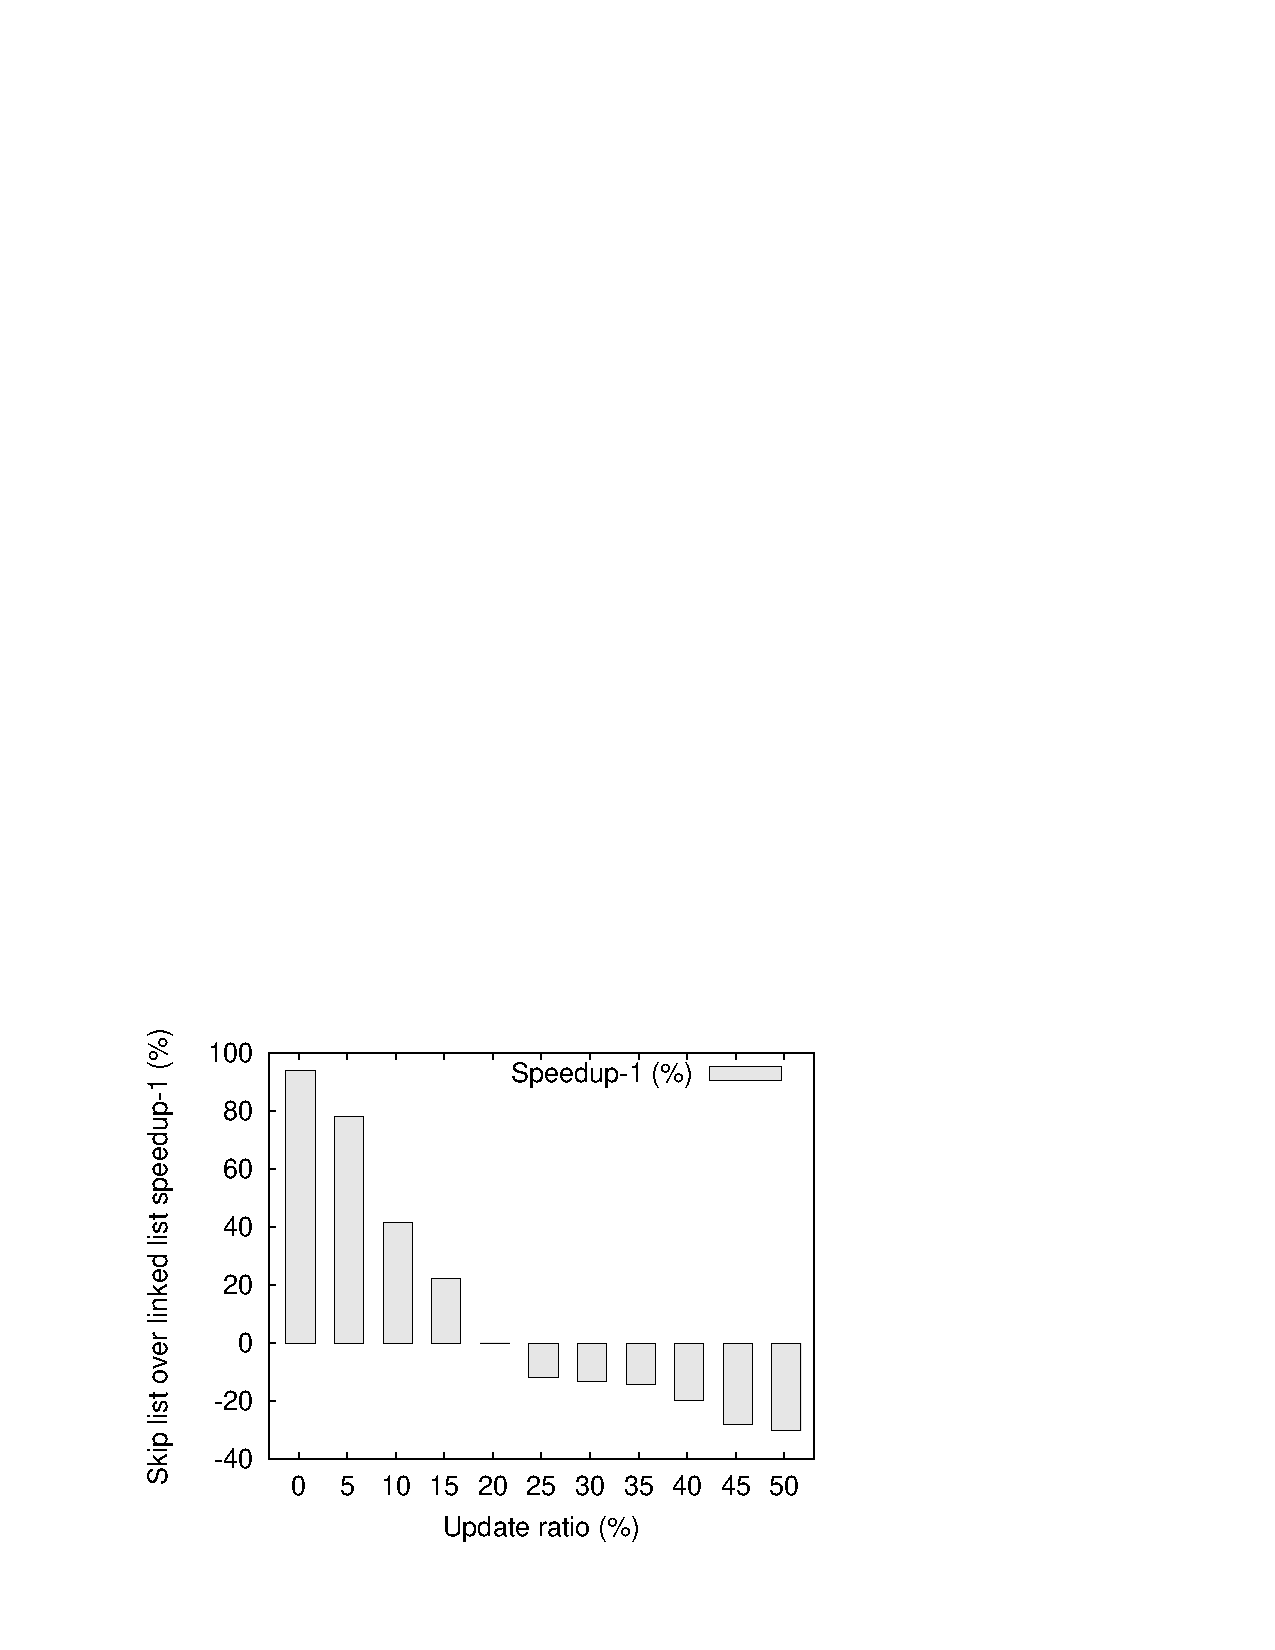
\includegraphics[scale=0.575,clip=true,viewport=50 50 400 300]{CF-general/fig/example}
	\caption{{\footnotesize Impact of contention on the performance of two 512-sized data structures (with 48 cores running with an increasing update ratio)\label{fig:contention}}}
\end{floatingfigure}

To better illustrate how contention can counterbalance the big-oh complexity  
in today's multi-/many-cores, Figure~\ref{fig:contention} depicts the performance
of a 48-core machine running the same set based experiment on a concurrent linked list, with $O(n)$ complexity,
and on a concurrent skip list, with $O(\log_2 n)$ complexity. 
A skip list, in short, is a structure that diminishes the complexity
of a linked list by being a sort of linked list 
%is a linked list 
whose nodes may have additional shortcuts pointing towards other nodes 
located further in the list~\cite{Pug90}. %(Skip lists are presented in Section~\ref{sec:sl}.)
%Figure~\ref{fig:contention} depicts the impact of contention on the performance of two integer set
%implementations, the first using a skip list offering a big-oh access complexity that is logrithmic in the 
%number of elements, the second using a linked list offering a linear access complexity.
In this experiment, 48 threads run insert/delete/contains accesses with an increasing proportion of 
update accesses over read-only ones on each of these two structures initialized with 512 
elements.\footnote{More precisely, this experiment was performed on a $4\times 12$-core AMD 
Opteron machine running at 2.1GHz and 32 GB of memory, each point is averaged 
over 5 runs of 5 seconds each, removes and inserts accesses are triggered with the same probability to keep the 
size expectation constant and removes/inserts that do not update the data structure are considered 
read-only accesses.}  To obtain the corresponding concurrent data structures used in the experiments, we simply encapsulated the 
sequential code of each access into an elastic transaction~\cite{FGG09}.
Interestingly, above 20\% updates the concurrent linked list is more efficient than the concurrent
skip list---this is shown by the negative values of the speedup-1. The reason is that the linked list 
updates are localized, that is, each of them only affects a constant number of nodes, typically the 
predecessor of the removed or of the newly inserted node. By contrast, the skip list updates 
may affect up to a logarithmic amount of predecessors for each removed of newly inserted node, 
producing additional contention.

This result is unsurprising as Herb Sutter noticed that linked list could better tolerate contention 
than balanced 
trees for similar reasons~\cite{Sut08}, yet it is interesting to observe experimentally that only 20\% 
updates make 
a linear complexity data structure better suited than a logarithmic complexity data structure on 
nowadays' multicore machines. 

In the light of the impact of contention on performance, we propose the \emph{Contention-Friendly (CF)}
methodology as a methodology to design new data structures that accommodate contention 
of modern multi-/many-core machines without relaxing the correctness of the abstractions.
To this end, we argue for a genuine decoupling of each access into an
eager abstract access and a lazy structural adaptation.
The abstract access consists in modifying the abstraction by minimizing the impact on the 
structure itself and aims at returning as soon as possible for the sake of responsiveness. 
The structural adaptation, which can be deferred until later, aims at adapting the structure to these changes by re-arranging elements or 
garbage collecting deleted ones.

We illustrate the CF methodology by designing three data structures with locks, universal primitives, and transactions: 
a skip list, a binary search tree and a hash table. 
As for the skip list, the aforementioned decoupling translates into splitting a 
node insertion into the insertion phase at the bottom level of a skip list and the structural 
adaptation responsible for updating pointers at its higher levels, or into splitting a node removal 
into a logical deletion marking phase and its physical removal and garbage collection.
Similarly, the decoupling of the binary tree accesses consists in inserting or logically removing a 
node prior to rebalancing and/or garbage collecting.
Finally, the hash table decoupling lies in inserting/deleting eagerly and resizing the structure lazily.

Our Java implementation of the resulting data structures indicates that our methodology leads to 
good performance on today's multicore machines. 
In particular using a micro benchmark, on a 64-way Niagara 2 machine our lock-based CF binary search tree improves 
the performance of the most recent Java lock-based binary 
search tree implementation~\cite{BCCO10} by up to $2.2\times$, our lock-based CF skip list 
improves the performance of Doug Lea's concurrent skip list adaptation of Harris and Michael algorithms~\cite{Har01,Mic02} by up to 
$1.3\times$, and our lock-free hash table outperforms by up to $1.2\times$ the JDK hash table, which is widely distributed in the $\lit{java.util.concurrent}$ package.
Finally, we show that state-of-the-art software transactional memories 
execute $1.5\times$ faster on average when the data structures are contention-friendly.

Section~\ref{sec:rw} describes the related work. Section~\ref{sec:cf} depicts the CF methodology, Section~\ref{sec:datastruct} illustrates it on three data structures. Section~\ref{sec:expe} presents the experimental results and Section~\ref{sec:conclusion} concludes. The companion appendix comprises the pseudo-code and correctness proofs of our CF algorithms, as well as additional experimentations using transaction-based variants of our CF algorithms and a discussion.

%
%\begin{abstract}
%In this paper, we propose a methodology to write speculation-friendly data structures.
%Although a lot of efforts were spent rethinking the transactional memory algorithms, 
%almost no efforts were spent rethinking the data structures accessed using transactions.
%
%Our methodology aims precisely at remedying this problem by listing the properties
%a data structure implementation should guarantee for speculative accesses to complete more rapidly.
%More specifically, this properties state that the same transactions should not comprise 
%abstract and structural modifications, that a structural modifications should be distributed 
%among sub-regions of the data structure, and that garbage collection should be acting 
%in the background independently from the actual logical removals.
%
%We illustrate this methodology with the first speculation-friendly library that comprises
%a binary search tree, a hash table, a linked list and a skip list.
%We show that this library outperforms the most efficient lock-based and lock-free alternatives 
%including the one of the Java concurrency package.
%Finally, we evaluate four state-of-the-art software TM libraries running on top of our library to show its portability.
%\end{abstract}
%
%\category{D.3.3}{Programming Languages}{Language Constructs and Features}[Concurrent programming structures]
%\category{E.1}{Data Structures}[Trees]
%\category{D.1.3}{Programming Techniques}{Concurrent Programming}[Parallel programming]
%\category{D.2.13}{Software Engineering}{Reusable Software}[Reusable libraries]
%
%\terms{Algorithms, Languages, Performance}
%
%\keywords{Abstract transaction, Structural transaction, Optimistic Concurrency, Transactional Memory}
%
%\section{Introduction}
%
%Multicore and manycore architectures are changing the way we write programs in three ways. 
%%{\bf Concurrency}
%First, every program, including irregular ones, should exploit concurrency thus all programmers must know how 
%to write a simple yet concurrent program.  
%%{\bf Contention Impact}  
%Second, the level of contention is expected to raise in irregular applications with the increasing number of 
%computational entities able to run concurrently, the cores, as they non-deterministically conflict when one process (thread) modifies a shared memory location another thread is accessing.
%%{\bf Resource Exploitation} 
%Third, the amount of cores at our disposal is expected to grow far beyond the traditional number of threads 
%we used to exploit, in part because reducing power consumption requires to simplify but multiply cores 
%
%To address the first challenge, speculative programming has proved effective in making concurrent programming modular~\cite{HHP05}: one can program a concurrent data structures another programmer can rely upon to simply derive her own 
%concurrent application.
%\vincent{What is speculation? Talk about Lampson's "Lazy and Speculative Execution in Computer Systems", Rachid's "Speculating Seriously", Idit's "Want scalable, speculate!", 
%Plan for the worst and optimize for the common: synchrony and low contention, but contention in many-core is expected to be quite high even at level of updates. Ravi Rajwar's thesis about multiprocessor speculation. Speculation for instructions, pipelining.}
%New programming constructs like transactions exploit this speculative approach~\cite{HM93,ST95}.
%Because transactions~\cite{HM93,ST95} cannot suffer from deadlocks, they encompass the drawback of trying to reuse
%lock-based data structures, and because they guarantee the atomicity of multiple accesses, they relieve the 
%programmer from the task of extending a library with hardware atomic primitives that apply to a single memory location.
%% transactions are appealing
%%New programming constructs like transactions have been suggested~\cite{HM93,ST95}.
%%Most transactions build upon \emph{optimistic synchronization}, 
%%where a sequence of shared accesses is executed speculatively and might abort.
%%They simplify concurrent programming for two reasons.
%The key concept of transactions is that the programmer only needs to delimit regions of sequential 
%code into transactions or to replace critical sections by transactions
%to obtain a safe concurrent program.
%%Second, the resulting transactional program is reusable by any programmer, 
%%hence a programmer composing operations from a transactional library into another 
%%transaction is guaranteed to obtain new deadlock-free operations that execute atomically.
%%By contrast, \emph{pessimistic synchronization}, where each access to some 
%%location $x$ blocks further accesses to $x$,
%%is harder to program with~\cite{PA11,RHW10} and hampers reusability.
%As a drawback of the simplicity of using transactions, 
%the existing transactional programs spanning from low level libraries to 
%topmost applications directly derive from program designed for non-speculative approach.
%
%\vincent{Cite Herb Sutter's Concurrency-friendly data structures.}
%We propose a speculation-friendly methodology to write highly efficient data structures 
%that reduce complexity of speculative accesses.
%This methodology generalizes the recent concepts of the speculation-friendly binary search 
%tree~\cite{CGR11} to arbitrary kind data structures to derive efficient libraries.
%Using this methodology, we propose four efficient data structures: a binary search tree, 
%a hash table, a linked list and a skip list.
%We show that a Java adaptation of our speculation-friendly binary search tree~\cite{CGR11} is more efficient 
%than the most recent concurrent tree alternative~\cite{}.
%In particular it is also more efficient than the $\lit{ConcurrentSkipList}$ from the Java concurrency package.
%More interestingly, we show that our new speculation-friendly skip list algorithm is even more efficient than 
%all these former algorithms. Besides being the most efficient logarithmic-complexity data structure known in Java 
%to date, it confirms that the speculation-friendly methodology is a powerful concept to obtain very efficient 
%data structures.
%
%The speculation-friendly methodology overcomes the two remaining modern challenges posed by the 
%multicore era.
%First, it limits contention by relaxing the existing data structure invariants without annihilating the abstraction semantics. Previous work on relaxing data structure invariants tends to weaken the semantics of the abstraction.
%For example, the Intel\textregistered{} Threading Building Blocks (TBB)\footnote{http://threadingbuildingblocks.org} relaxed the FIFO policy of the queue with multiple consumers/producers. Recent proposals~\cite{Sha11} tend to trade similar guarantees to obtain highly concurrent stacks.
%
%% problem
%The problem of adapting data structures for speculative execution remains vastly unexplored 
%though our recently published binary search tree~\cite{CGR12} clearly motivates the importance of such a topic.
%Pessimistic operations must typically guarantee some invariants about the location of nodes in 
%the structure. These invariants help ensure that the complexity of
%searching a given element is always upper-bounded, guaranteeing the step complexity.
%To preserve these invariants,
%an operation affecting the structure by removing, inserting or simply moving nodes
%must additionally check whether its modification affects the invariants. If so, it must then execute a dedicated \emph{restructuring}, 
%a process that modifies the data structure without modifying the state of the abstraction it implements, to compensate the modification 
%and preserve the invariants.
%The modification and its compensating restructuring must naturally appear to be executed \emph{atomically}, 
%in a single indivisible step from the standpoint of the system, to make sure the transient invariant violation 
%is not visible from further operations.
%
%
%However, the resulting complexity really depends on the type of synchronization.
%The complexity of pessimistic concurrency control is tied to the number
%of protected steps that are guaranteed to complete despite blocked 
%attempts of interfering, whereas the complexity in optimistic concurrency 
%control is tied to the number of speculative attempts that fail due to 
%unavoidable interferences.
%Put simply, while a pessimistic update on a data structure 
%tries to minimize the number of its successful protected steps, the 
%optimistic one should rather minimize its unsuccessful speculative steps.
%
%% state of the art
%Currently, three techniques exist to boost the performance of the transactions used to access 
%data structures.
%%Currently, three major research directions are explored to  
%%obtain efficient transactional executions on data structures.
%First, high-level conflict detection aims at ignoring the low-level 
%conflicts of structural transactions by using abstract 
%locks~\cite{Mos06,NMA+07,CMC07,HK08,ALS09}.
%Second, various language extensions have been
%proposed as escape mechanisms within a transaction 
%to limit the transaction bookkeeping~\cite{HLMS03,CH05,FGG09,AMT10}. 
%The former approach exploits the application semantics and cannot 
%be automated while the latter approach requires the programmer
%to tune the underlying TM implementation generally not supported 
%by TM compilers~\cite{abi}. 
%Third, the combination of various transaction semantics cope with unsupported
%language extensions~\cite{FGG09,GG11} but still puts the burden of choosing the 
%right semantics on the programmer.
%The idea of boosting the speculatively accessed data structure itself has just been suggested
%but we only evaluated binary search trees~\cite{CGR11} and ignore whether it can be applied to other
%data structures. 
%
%% contributions
%We propose a methodology to write \emph{speculation-friendly data structures}. In short, it consists in relaxing transiently their structural invariants without hampering the abstraction consistency in order to speed up transaction-based accesses.  
%We illustrate this methodology through a speculation-friendly library that comprises four data structures:
%a binary search tree, a hash table, a linked list and a skip list. The characteristics of these new algorithms 
%are as follows:
%\begin{itemize}
%	\item {\bf Binary search tree.}
%We verify that our previous binary search tree~\cite{CGR12} respects the methodology.
%In particular we implemented an object-based version in Java of our previous C implementation to evaluate
%its performance against the performance of the latest (after ours) binary search tree algorithm~\cite{BCCO10}. We show that our resulting algorithm is \vincent{TODO}$\times$ faster than the most recent tree algorithm, and \vincent{TODO}$\times$ faster than the skip list  $\lit{java.util.concurrent}$ package (the only propose data structure with logarithmic access complexity).
%	\item {\bf Linked list.}
%We propose a new linked list algorithm that is speculation-friendly in that is decouples the logical and physical 
%removal process 
%As linked list data structures have the appealing aspects of supporting localized updates, its performance benefit is marginal compared to other data structures. \vincent{Maybe compare against synchronizedSet Linked List?}
%	\item {\bf Hash table.} 
%We propose a new hash table algorithm that is speculation-friendly in that its resize operation is done in the background rather than being part of an update operation that exceeds the maximal tolerated load.
%In addition, we reuse our speculation-friendly linked list algorithm to implement each independent bucket.
%	\item {\bf Skip list.}
%We propose a new skip list algorithm that is speculation-friendly in that the structural level of each node are adapted in the background rather than being tightly coupled with the corresponding insert operation.
%We compare our skip list performance against the $\lit{java.util.concurrent}$ skip list and our speculation-friendly tree algorithm. Perhaps surprisingly, this data structure is the most efficient data structure we have observed.
%\end{itemize}
%Finally, we also evaluate a version of the speculation-friendly library as part of the bytecode instrumentation 
%framework Deuce~\cite{KSF10}. Although this framework adds a significant overhead to the execution time, it greatly 
%simplifies the usage of various transactional memory algorithm. We report on the performance of 
%TL2~\cite{DSS06}, LSA~\cite{RFF06}, ${\mathcal E}$-STM~\cite{FGG09},  NOrec~\cite{DSS10} when running 
%speculation-friendly data structure and in particular we illustrate the 
%portability of our library to TM systems satisfying the standard TM interface~\cite{abi}.
%
%%Ok, for the tree we should keep in mind that:
%%- the background rotating thread was originally proposed by Mander and Ladner in 1984 
%%- the distributed rotation (w/ propagation) was proposed by Bouge et al. in 1998
%%- the separate garbage collector was proposed by Dijkstra et al. in 1978
%%But the novelty is to decouple *speculative* operations.

\section{Related Work}\label{sec:rw}

Various complexity metrics exist to evaluate data structures efficiency on a given workloads. 
% big-oh notation in theory
From a theoretical point of view, the big-oh notation helps to derive data structures whose access step 
complexity is proportional to the total number of elements.
Typically, balanced trees have a logarithmic big-oh access complexity whereas non-overloaded hash 
tables have a constant big-oh access complexity.
This big-oh complexity does not capture the cost of contention and theoretical models have been 
explored to remedy this issue~\cite{DHW97}. Unfortunately, there are not enough evaluations of this 
impact in practice. 

% locality in practice
From a more pragmatic point of view, the locality of data both in terms of space (i.e., the promiscuity of 
data stored in memory) and time (i.e., 
the closeness of the points in time at which they are accesses) has been an important metric of 
consideration when implementing data structures in cache-coherent systems.
Cache-aware and cache-oblivious data structures try to exploit locality to maximize the chance of cache 
hits. While the former data structures rely on some tunable parameter that can accommodate the 
targeted platform like the Judy array\footnote{\texttt{http://judy.sourceforge.net}}, the later aims at being 
more portable by flattening cleverly structural nodes into memory~\cite{FLPR99}, for example the tree algorithm 
of van Emde Boas et al.~\cite{vEKZ76}. Both approaches are tied to cache-coherent machines but do 
not accommodate upcoming many-core platforms whose cache-coherence is either 
limited~\cite{WGH+07} or absent~\cite{MRL+10}. 
%In particular, this observation led researchers to 
%rethink even existing shared-memory cache-coherent machines in terms of distributed systems, where threads communicate by sending inter-core messages instead 
%of assuming a simplifying but costly shared memory~\cite{BBD+09}.

The decoupling of the update and rebalancing was vastly explored in the context 
of trees~\cite{GS78,Kes83,NSW87,NS98,UR84,IRISAppr,Bal06,CGR12} 
%Various database trees where proposed with a decoupling of update and 
%rebalancing~\citep{GS78,Kes83,NSW87,NS98,UR84,IRISAppr} 
but this idea was 
not generalized to other search structures.
The decoupling of the removals in logical and physical phases was originally studied in transactional systems~\cite{Moh90}
and later applied to various lock-free data structures including linked lists~\cite{Har01}, hash tables~\cite{Mic02}, skip lists~\cite{Fra03,FR04} and binary search trees~\cite{EFRB10}
but insertions in these data structures were not decoupled.
The contention friendly methodology generalizes these decoupling into an eager abstract access and a lazy structural adaptation that benefit
both insertions and removals.

Our methodology is independent from the synchronization primitive used but lies essentially in splitting 
accesses into an eager abstract access and a lazy structural adaptation.
Although we focus essentially on lock-based data structures, we also evaluate the benefit of various
transactional memory algorithms when running our contention-friendly data structures.
We have already illustrated the benefit of decoupling accesses into separate transactions 
in~\cite{CGR12} on a C-based 
binary search tree.  In such optimistic executions, this decoupling translated into avoiding a conflict with a 
rotation from rolling back the preceding insertion/removal.
Here we generalize our previous work by showing how a similar decoupling can benefit 
pessimistic execution and various search structures and we compare our results to existing Java concurrent structures.
%We generalize our previous work to pessimistic executions and by experimenting our methodology on several Java-based STM algorithms 
%and additional contention-friendly data structures.
Previous investigations on improving the performance of transaction-based data structures focused 
exclusively on the improvement of the transaction algorithm. Some of these investigations led to the 
development of novel transaction models based on abstract locks to ignore low level conflicts~\cite{NMA+07,HK08}, 
or elastic transactions~\cite{FGG09}.

Finally, Shavit suggests to relax data structure guarantees in the light of the new multicore context~\cite{Sha11}. A stack algorithm and several relaxations to this algorithm
are presented to support concurrency. The objective as well as the means to achieve it are quite different from ours. 
First, the problem raised by placing the stack into the multicore context is that performance drops below the sequential stack performance, and 
the goal is to diminish contention to limit this concurrency drawback. By contrast, we focus on deriving alternative data structures that are more scalable than highly concurrent ones, hence leveraging multi-/many-cores.
Second, the goal of limiting contention induced by multiple cores is achieved by relaxing consistency. In the stack example, this relaxation boils down 
to replacing linearizability by quiescent consistency, guaranteeing that the last-in-first-out policy of an access is only with respect to preceding calls 
when no other accesses execute concurrently.
Conversely, the contention friendly methodology aims at replacing existing data structures without relaxing their abstraction consistency: all accesses remain linearizable.

%\vincent{We should talk about the java.util.concurrent package that some decoupling with lazy techniques. At least explain the difference with concurrentHashMap and ConcurrentSkipListMap/Set.}

\section{The CF Methodology at a Glance}\label{sec:cf}

%The Contention-Friendly (CF) Methodology relies on several observations on speculative execution: (i)~multicore raises contention that impacts sometimes more the execution complexity than the structure itself; (ii)~multi/many-cores provide more computational resources than we used to exploit.
In this section, we give an overview of the Contention-Friendly (CF) methodology by describing how to write contention-friendly data structures.

The CF methodology aims at modifying the implementation of existing data structures using two simple rules without relaxing their correctness. The correctness criterion ensured here is linearizability~\cite{HW90}.  The data structures considered are \emph{search 
structures} because they organize a set of items referred to as \emph{elements} in a way that allows to retrieve the unique expected position of an element given its value. 
The typical abstraction implemented by such structures is a collection of elements that can be specialized into various sub-abstractions like a set (without duplicates) or a dictionary (that maps each element to some value). We consider \emph{insert}, \emph{delete} and \emph{contains} operations 
that respectively inserts a new node associated to a given value, removes the node associated to a given value or leaves the structure unchanged if no such node is present, and returns the node associated to a given value or $\bot$ if such a node is absent. Both inserts and deletes are considered \emph{updates}, even though they may not modify the structure.

\begin{table*}
\begin{center}
{\footnotesize
\renewcommand{\tabcolsep}{1pt}
\renewcommand{\arraystretch}{1}
\begin{tabular}{|l|l|l|l|}%{|l|l|rl|}
  \hline
  {\bf Data structure} & {\bf Invariant} & {\bf Abstract modifications} & {\bf Structural adaptations} \\ \hline\hline

  {\bf Hash tables} & constant load factor & key-value pair insertion & adding buckets and rehashing \\
  & (i.e., $\#\lit{nodes} / \#\lit{buckets} = O(1)$) & logical deletion & physical deletion + rehashing\\ \hline
  %{\bf Linked lists} & linear access time complexity (i.e., $O(n)$)& logical deletion & physical deletion \\ \hline
    {\bf Search trees} & balance & node insertion & rotation \\
  & (i.e., shortest route to leaf $\approxeq$ longest route to leaf) & logical deletion & physical deletion + rotation \\ \hline
  {\bf Skip lists} & node distribution per level & horizontal insertion & vertical insertion + increasing toplevel \\
  & (i.e., $\Pr[\ms{level}_i=j] = 2^{O(j)}$) & logical deletion & physical removal + decreasing toplevel \\ \hline
\end{tabular}}
\end{center}
\vspace{-1.5em}
\caption{\footnotesize Decoupling example of existing data structure accesses into an abstract modification and a structural adaptation\label{table:restructuring}}
\end{table*}
%\vspace{-1em}

%The first rule 
The key rule of the methodology is to decouple each update into an \emph{eager abstract modification} and a \emph{lazy structural adaptation}. The secondary rule is to make the removal of 
nodes selective and tentatively affect the less loaded nodes of the data structure.
These rules induce 
%This requires 
slight changes to the original data structures as summarized in Table~\ref{table:restructuring}, that result in a corresponding 
data structure that we denote using the \emph{contention-friendly} adjective to differentiate them 
from their original counterpart.

\vspace{-1em}
\subsection{Eager abstract modification}

Existing search structures rely on strict invariants (cf. Table~\ref{table:restructuring}) to guarantee their big-oh complexity, hence each 
time the structure gets updated,  the invariant is checked and the structure is accordingly 
adapted instantaneously. While the update may affect a small sub-part of the abstraction, 
its associated restructuring is a global modification that conflict potentially with any concurrent update, 
thus increasing contention.
 
The CF methodology aims at minimizing such contention by returning eagerly the modifications of the 
update operation that makes the changes to the abstraction visible. By returning eagerly, each 
individual process can move on to the next operation prior to adapting the structure. It is noteworthy 
that executing multiple abstract modifications without adapting the structure does no longer guarantee the big-oh step complexity of the accesses, yet such complexity may not be the predominant factor in 
contended execution as we reported in the Introduction.

A second advantage is that removing the structural adaption from the abstract modification makes the cost of each operation more predictable.  All operations share similar cost and create the same amount of contention.
%whereas
%in existing data structures for example one insert in a tree might require $O(\log(n))$ rotations while 
%another
%insert might not require any rotation, leading to unpredictable response time.
More importantly the completion of the abstract operation does not depend on the structural adaptation
(like they do in existing algorithms) 
so the structural adaptation can be performed differently, using and depending on global information.
%This means that the adaptations can be preformed differently without directly impacting the abstract operations.
%For example the modifications can use global information or be more costly than they are in existing algorithms

\vspace{-1em}
\paragraph{The skip list example.}

A traditional skip list picks a level for each node when they are
inserted based on some pseudo-random function.  The aim of this function
is to distribute the levels so that operations have an average cost of
$O(\log{n})$.  In certain workloads this can be preferred over trees due
to the assumption that rotations are more costly. 
When a node is inserted in
the contention-friendly skip list it has a level of one, which is all that is needed to ensure the correctness of the abstraction.

\begin{floatingfigure}{7.5cm}
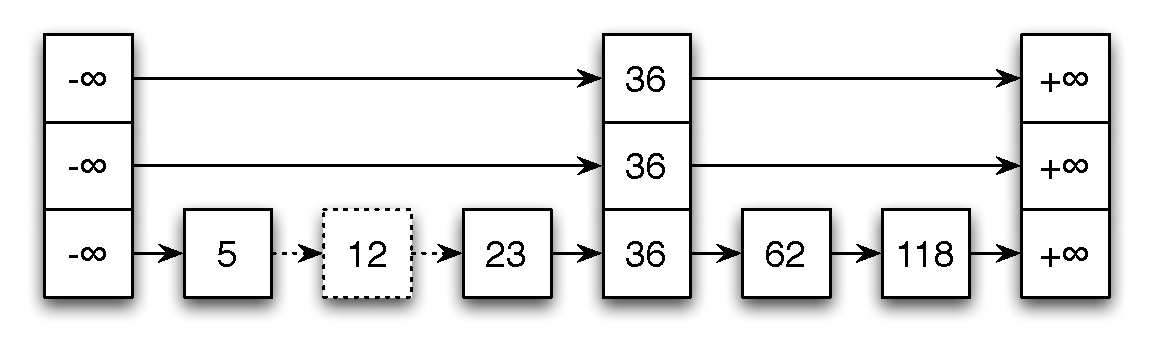
\includegraphics[scale=0.35]{CF-general/fig/horizontal-insert}
%\vspace{-1em}
\caption{\footnotesize{Inserting horizontally in the skip list\label{sfig:horizontal}}}
\end{floatingfigure}

As an example, assume we aim at inserting an element with value 12 in a skip list.  Our 
insertion consists in an abstract modification that updates only the bottom most level by inserting the new 
node as if its level was the lowest one leading to Figure~\ref{sfig:horizontal} where dashed arrows indicate the freshly modified pointers.
We defer the process of linking this same node at higher levels, to diminish 
the probability of having this insertion conflict with a traversing operation.

\subsection{Lazy structural adaptation}

The purpose of decoupling the structural adaptation from the preceding abstract modification is to enable its postponing (by, for example, dedicating a separate thread to this task), hence the term ``lazy'' structural adaptation.
The main intuition here is that this structural adaptation is intend to ensure the big-oh complexity rater 
than to ensure correctness of the state of the abstraction.
Hence, the linearization point belongs to the execution of the abstract modification and not the structural 
adaptation and postponing the structural adaptation does not change the effectiveness of operations.
The visible modification applied to the abstraction (and the structure) during the abstract modification guarantees that any further operation applying to the same structure will observe the changes. This helps ensuring that all operations are linearizable in that real-time precedence is 
satisfied. In Appendix~\ref{sec:proof} we show that our structures implement a linearizable abstraction. 

This postponing has several advantages whose prominent one is to enable merging of multiple
adaptations in one simplified step. Although the structural adaptation might be executed in a 
distributed fashion, by each individual updater threads, one can consider centralizing it at one 
dedicated thread.
Since these data structures are designed for architectures that use many cores
performing the structural adaptation on a dedicated single separate thread, takes advantage of 
hardware that might otherwise be left idle.
Only one adaptation might be necessary for several abstract modifications and minimizing the 
number of 
adaptations decreases accordingly the induced contention. Furthermore, several adaptations can 
compensate each other as two restructuring can lead to identity. For example, a left rotation executing 
before a right rotation at the same node may lead back to the initial state and executing the left rotation 
lazily makes it possible to identify that executing these rotations is useless.

\paragraph{The skip list example.}

As explained in the previous example the insertion executes in two steps. Once the horizontal 
insertion of node 12, depicted in Figure~\ref{sfig:horizontal}, is complete, a restructuring is necessary to 
ensure the logarithmic  complexity of further accesses. 
\begin{floatingfigure}{7.5cm}
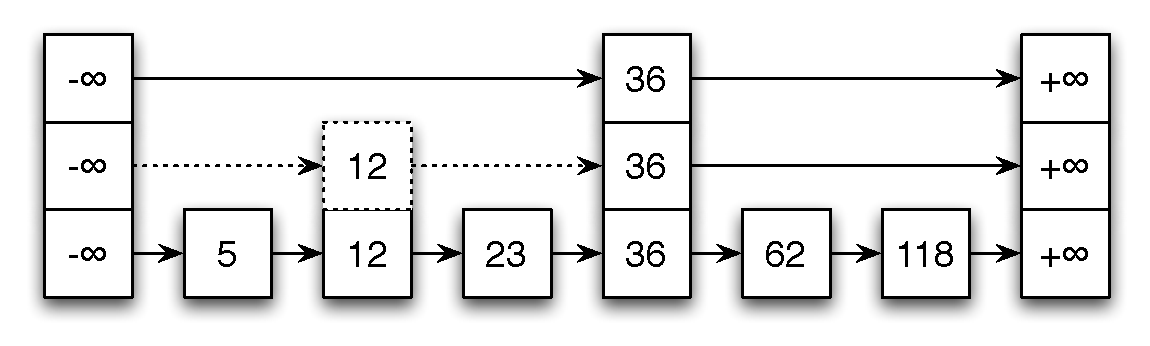
\includegraphics[scale=0.35]{CF-general/fig/vertical-insert}
%\vspace{-1em}
\caption{\footnotesize{Adapting vertically the skip list structure\label{sfig:vertical}}}
\end{floatingfigure}

A separate structural adaptation step is accordingly raised to increase the node level appropriately.
%In a tree the physical insertion is decoupled from any necessary rotations.
%In a hash table insertion is decoupled from any resizing and rehashing operations.
The insertion at higher levels of the skip list is executed as a separate step, which guarantees 
eventually a good distribution of nodes among levels as depicted in Figure~\ref{sfig:vertical}.
This decoupling allows higher concurrency by splitting one atomic operation into two atomic operations.

\subsection{Selective removal}
In addition to decoupling level adjustments, we do selective removals.
A node that is deleted is not removed instantaneously, instead it is
marked as deleted.  The structural adaptation then selects cleverly nodes that
are suitable for removal, i.e., whose removal would not induce high contention.
This is
important because removals may be expensive.  
Removing a frequently accessed node
requires locking or invalidating a larger
portion of the structure.
%In the worst case this node would be the root of a tree or the tallest
%node in a skip list.
Removing such a node is likely to cause much more contention
than removing a less frequently accessed one.
In order to prevent this, only nodes
that are marked as deleted and have a level of 1 (in the skip list) or 
a single or no children (in the tree) are removed.
This leads to less contention, but also means that certain nodes that are marked as deleted will not be removed.
In the tree it has already been observed that only removing such nodes~\cite{CGR12},\cite{BCCO10} results in a similar sized structure
as existing algorithms.
In the skip list the level of a node is calculated in such a way that after a structural adaptation is performed less than
half the nodes (in the worst case) in the list will be marked as deleted.
In practice this number is observed to be much smaller.

\paragraph{The skip list example.}
Let us look at a specific example with the skip list.
On the one hand, a removal of a node with a high level, say the one with value 36 in 
Figure~\ref{sfig:vertical}, would typically induce more contention than the removal of a node with a lower 
level, say the one with value 62 spanning a single level.
The reason is twofold. First removing a node spanning $\ell$ levels boils down to updating $\ell$ 
pointers which increase the probability of conflict with a concurrent operation accessing the same 
pointers, hence removing node with value 36 requires to update 3 pointers while node with value 63 
requires to update a single pointer. Second, the organization of the skip list implies that higher level 
pointers are more likely accessed by any operation, hence the removal of 36 
typically conflicts with every operation concurrently traversing this structure (because all these 
operations would follow the topmost left pointer) whereas the single next pointer of 62 is unlikely accessed by concurrent traversals.
Removing a tall node such as 36 would also mean that in order to keep the logarithmic complexity of the traversals a
node would have to take its place at an equivalent height.

%\vincent{Talk about distribruted vs. centralized restructuring}
%The final advantage is thanks to the multicore hardware.
%Even though the structural adaption is done separately, someone stills need to do them so that the abstract operations remain efficient.
%Since these data structures are designed for architectures that use many cores the structural adaptations are performed entirely by a separate thread,
%taking advantage of hardware that might otherwise be left idle.

\subsection{Avoiding contention during traversal}
Each abstract operation ($\ms{contains}$, $\ms{insert}$, $\ms{delete}$) of a tree or a skip list is %not so different from in an existing sequential algorithm.
%They are each
expected to traverse $O(\log{n})$ nodes.
Given that the traversal is the longest part of the operation, the CF algorithms try to avoid as often as possible producing contention.
%
Concurrent data structures often require more complex synchronization operations during traversal (not including the updates done after the traversal).
% Such as
For example, locking nodes in a tree helps ensure that the traversal remains on track during a concurrent rotation~\cite{BCCO10}, using $\lit{compare-and-swap}$ operations during traversal helps the raising and lowering of levels of a concurrent $\ms{insert/delete}$ in a lock-free skip list~\cite{Fra03}, or using optimistic strategy helps at the risk of having to restart~\cite{HLL07,HS08}.

Usually these synchronization operations are required due to structural adaptations and the CF 
algorithms structural adapt differently to especially so that operations can avoid using
locks or synchronization operations during traversal.
%
\remove{
The structural adaptations are also designed to avoid contention where possible.
This means applying the selective removal of nodes that are traversed less 
frequently, as well as using locks/synchronization as little
and as localized as possible. For example, only reads/writes are used when modifying the upper levels of the CF skip list, rotations in the CF tree are performed as localized
operations, and rehashing of the CF hash table is done per bucket.
}

\section{Putting the CF Methodology to Work}\label{sec:datastruct}

Here we present how we apply the contention-friendly (CF) methodology to three data structures. For further detail on the algorithms and correctness proofs please refer to Appendix~\ref{app:pseudocode}
and Appendix~\ref{sec:proof}, respectively.


%\subsection{CF Tree and Skip list}

\subsection{CF Skip list}

The CF skip list is made up of several levels of linked lists,
with the bottom level being a doubly linked list.
Each node on the bottom level contains the following fields:
A key $k$, a $\ms{next}$ and $\ms{prev}$ node pointers, a lock field, a $\ms{del}$ flag indicating 
if the node has
been marked deleted, and a $\ms{rem}$ flag indicating if the node has been physically removed.
The algorithm presented here is lock-based, however, we have derived a transaction-based version
(cf. Appendix~\ref{sec:tm}).
% relaxing structural invariants
%As the complexity of speculative execution does not only depend on the distribution of levels of the skip 
%list nodes but also on the contention, we aim at minimizing both instead of focusing on the ideal 
%distribution. Specifically, we trade transiently the ideal distribution of levels to diminish 
%contention of speculative accesses by avoiding updating the higher levels as part of the update 
%operation.
%
%Transactionalizing a skip list implementation, be it sequential with no 
%synchronization technique or concurrent using locks for synchronization purpose, would naively result 
%in encapsulating each update operation into a dedicated transaction, yet this update would  typically do several things.

%\begin{figure}[ht!]
%\begin{center}
%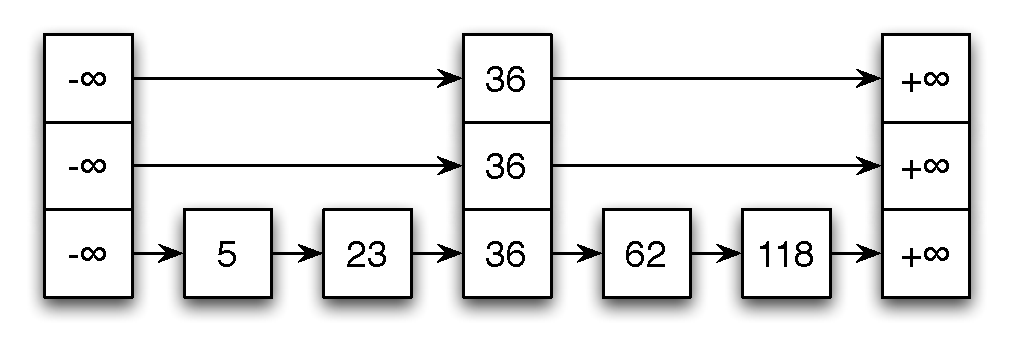
\includegraphics[scale=0.45]{fig/skiplist}
%\caption{A skip list example where removing node 62 induces more contention than removing node 36\label{fig:sl-remove}}
%\end{center}
%\end{figure}


\remove{
On the other hand, an insertion operation, say of value 12 with no loss of generality, as depicted in Figure~\ref{fig:sl-insert} would typically insert \emph{horizontally} a new node at the bottom level of the skip list 
(Figure~\ref{sfig:horizontal}) but also update \emph{vertically} the higher levels to 
guarantee that further operations have a logarithmic complexity (Figure~\ref{sfig:vertical}). 
The horizontal phase is both a structural and an abstraction modification: once executed the 
state of the abstraction reflects the changes. By contrast, the vertical phase is only a structural 
adaptation that does not impact the state of the abstraction.
% rewording
In other words, inserting the node at the bottom level guarantees that the node is 
reachable and that the value is part of the abstraction. Updating the higher 
levels is only necessary for efficiency purpose, not for safety purpose. 
}

\remove{
Motivated by the fact, that future multicore will provide more and more cores, we 
aim at exploiting additional cores (at least one) responsible of maintaining the 
data structure in the background.
}
\paragraph{Abstract operations.}
The goal of these CF algorithms is for the abstract operations
 to encounter and produce as little contention as possible.
%
In particular, it boils down to 
%As previously discussed this means deletions are done by 
setting the nodes
$\ms{del}$ flag to $\lit{true}$ to delete a node 
as well as linking 
%insertions only insert 
a new node to the bottom list level to insert it.
These modifications are necessary to guarantee that
linearizability, with all other structural adaptations being saved for later execution.
For the sake of safety, the abstract insertion acquires a lock on the predecessor 
node of the to-be-inserted node whereas the abstract deletion acquires a lock 
on the to-be-marked node. The lock is immediately released after the insertion 
or deletion completes. 
%In order to ensure
%these operations are able to execute safely they lock the node they modify.
%For the insert this is the node previous to where the new node will be inserted
%and for the delete this is the node that will be marked as deleted.

No locks are acquired during the traversal, inducing no contention.
%In order to avoid contention during traversal,  no locks are acquired.
More precisely, while traversing upper levels the operation will move forward in the list using
the $\ms{next}$ pointer until it encounters a node with a larger key than the one being search for
at which point it will move down a level, similarly to a bare sequential implementation would do.
At the bottom level the traversal may end up on a node that is physically removed due
to a concurrent structural adaptation $\ms{remove}$ operation, in this case it travels backwards in the list
following the $\ms{prev}$ pointer until it arrives at a node that has not yet been removed.
%by updating as many pointers as its level. By contrast, a removal of node with a lower level, say the one with value 63 in Figure~\ref{fig:sl-insert} spanning a single level, would simply require to update a single pointer. 

\paragraph{Structural adaptation.}

The first task of the structural adaptation is to remove nodes marked as deleted
who have a height of $1$.
In order to prevent conflicts with concurrent abstract operations
the node $\ms{n}$ to be removed and its predecessor in the list ($\ms{n.prev}$) are locked.
The prior nodes $\ms{next}$ pointer ($\ms{n.prev.next}$) is then modified so that it points to the next 
node ($\ms{n.next}$), and the next node's $\ms{prev}$ pointer ($\ms{n.next.prev}$) is then modified to point to the previous node ($\ms{n.prev}$).
Finally the $\ms{n}$'s $rem$ flag is set to true and the locks are released.

The structural adaptation must also modify the level of nodes in order to ensure
the $O(\log{n})$ expected traversal time.
Since neither removals nor insertions are done as they are in traditional skip lists,
calculating the height of a node must also be achieved differently.
Existing algorithms call a random function to calculate the heights of nodes, but
if this same function was used here the structure would end up with
excessive tall nodes.

When choosing the heights it is important to consider that
the fundamental structure of a skip list is not designed
to be perfectly balanced but rather probabilistically balanced.  
Consider a perfectly balanced skip list.  The node in the very middle of the list would
be the tallest node and the nodes just to the right and left of this
node would be nodes with height $1$.  Now if a couple new nodes are
inserted at the very end of the list then to
re-balance the skip list the node that was previously the tallest
node would now be shrunk to a level of $1$, and one of its
neighboring nodes which previously had height of $1$ would become the tallest node.
Instead a scheme of approximately balanced is more fitting for the skip list
(as this is what the existing algorithm's random functions do).

By contrast, the CF skip list deterministically adjusts the level of nodes.
%The contention friendly algorithm uses the following
%procedure to adjust the heights of the nodes.
From the bottom level going upwards, it traverses the entire list of the level, 
and each time it observes that 3 consecutive nodes whose height equals this level,
it raises the level of the second of this node (the one in the middle) by 1.
%Starting from the bottom level going upwards, do the following at
%each level:
%Traverse the entire level.
%Each time $3$ nodes in a row of height equal to the current level
%are encountered, raise the level of the middle of these nodes by $1$.
Such a technique approximates the targeted number of nodes present at each level, 
balancing the structure.
%This creates an approximate correct number of nodes at each level
%and creates an approximately correct balance.
Doing this is similar to the original intuition of the skip list, there is no
frequent re-balancing going on, tall nodes will stay tall nodes.
Less modification of the taller nodes also means less contention
at the frequently traversed locations of the structure.

Given that the number of nodes in the list might also shrink
the height of nodes might also be lowered.
When the height of the tallest node is greater than some threshold
(usually when the height is greater than the $\log$ of the total number of
nodes in the list) the entire bottom index level of the skip list is simply removed
by modifying the $\ms{down}$ pointers of the level above.
Doing this avoids constant modification of the taller nodes and ensures
there are not too many marked deleted nodes left in the list.

\subsection{CF Tree}

The CF tree is a binary search tree. Each of its nodes contains the following fields: a key $\ms{k}$, pointers $\ms{l}$ and $\ms{r}$ to the left and right children nodes, a lock field, a $\ms{del}$ flag indicating if the node has
been marked deleted, and a $\ms{rem}$ flag indicating if the node has been physically removed.
As for the CF skip list, the CF tree algorithm presented here is lock-based but we also derived 
a transaction-based variant of it.

\paragraph{Abstract operations.}
Similarly to the CF skip list operations the 
$\ms{insert}$ and $\ms{delete}$ operations must acquire a lock on the node
they modify.
A $\ms{delete}$ operation sets the node's $\ms{del}$ flag to $\lit{true}$ while an $\ms{insert}$ operation allocates a new node and modifies the parent's child pointer to point to it.

The traversal is performed without locks.
At each node the traversal travels to the right child if the node's key is larger than $k$,
otherwise it travels to the left child.
Since locks are not used, the traversal might get caught during a concurrent removal or rotation, but
the structural adaptation is done in such a way that
the traversal can continue safely following the child pointers.

\paragraph{Structural adaptation.}
The structural adaptation is in charge of removing marked deleted nodes that have
at most one non-$\bot$ child pointer.
Removals are done by first locking the node $n$ to be deleted and its parent.
The parent's child pointer is then modified so that it points to $n$'s non-$\bot$
child (if any).
Next $n$'s child pointers are modified so that they point upwards to it's parent node
allowing concurrent traversal that arrived on this node a safe path back to the tree.
Finally $n$'s $\ms{rem}$ flag is set to $\lit{true}$ and the locks are released.

The structural adaptation must also perform rotations in order to ensure the tree is balanced
so that traversal can be done in $O(\log{n})$ time.
Methods for performing localized rotation operations in the binary trees have already been examined and proposed
in several works such as ~\cite{CGR12,BCCO10}.
The main concept used here is to propagate the balance information from a leaf to the root.
A leaf is known to have height of $0$ for their left and right children.
This information is then propagated upwards by sending the height of the child to the parent where the value
is then increased by $1$.
Local rotations are performed depending on this information and result eventually in a balanced tree.

In order to avoid using locks and aborts/rollbacks during traversals, rotations are performed differently than traditional rotations.
Before performing the rotation the parent node and its child node that will be rotated are locked in order to
prevent conflicts with concurrent $\ms{insert}$ and $\ms{delete}$ operations.
In a traditional rotation there is one node $\ms{n}$ that is rotated downwards and one node (one of $\ms{n}$'s children)
that is rotated upwards.
A traversal preempted on the node rotated downwards ($\ms{n}$ in this case) is then in danger of being set off track and missing the
node it is searching for.
The rotations performed in the CF algorithm avoid this by not actually rotating $\ms{n}$ at all,
meaning that after the rotation $\ms{n}$ still has a pointer to the node that is rotated upwards allowing traversals to continue safely.
Instead a new node takes $\ms{n}$ place in the structure.
This new node is set to have the same values and pointers as $\ms{n}$ would if a rotation was performed as normal.
After the rotation, the node $\ms{n}$ has its $\ms{rem}$ flag set to $\lit{true}$ 
%as it is no longer in the tree.
and, finally, the locks are released.

\remove{
The main difference between the algorithm presented here is the decoupling of these operations.
The second difference is a slightly more complicated rotation procedure is used here
(but since they are performed separately, they do not slow the abstract operations).
This modified rotation procedure allows concurrent traversals to pass rotated nodes without having to use
synchronization methods.
A description of the rotations can be found in section \cite{sec:treemaint}.
}

\subsection{CF Hash table}

The CF hash table contains an array of pointers with each location pointing to $\bot$ or to
a list of nodes. Each node contains the following fields.
A key $\ms{k}$, and a $\ms{next}$ pointer pointing to the next node in the list.
This algorithm is lock-free (relying on $\lit{compare-and-swap}$ for synchronization) but we derived a transaction-based variant of it (cf. Appendix~\ref{sec:tm}).

\paragraph{Abstract operations.}

Given that the traversal for the $\ms{contains}$, $\ms{insert}$, $\ms{delete}$ operations has complexity $O(1)$ and not $O(\log{n})$ the
hash table operations are performed slightly differently.
In fact, the shortness of the hash table operations brings two main differences to the algorithm.

First physical removals are done from within the $\ms{delete}$ operation.
This is because the contention caused by removing the node will only be with other nodes of that bucket which are expected to be
$O(1)$.

Second the algorithm is made lock-free because given the short operations, a cache miss caused 
by loading a lock could be relatively costly.
Other implementations might avoid this by using coarser grained locks, like lock-striping, but
this can cause contention on the lock(s).
Instead we use a lock-free implementation where each operation only uses (at most)
a single synchronization operation, which is a $\lit{compare-and-swap}$ on the given bucket pointer.

For the sake of linearizability of operations the $\lit{compare-and-swap}$ always happens
at the same location (on the bucket pointer) and the $\ms{next}$ pointer of list elements
is never modified after node creation.
An $\ms{insert}$ will $\lit{compare-and-swap}$ a new node as the first element of the list, while
a $\ms{delete}$ will remove a node by creating a new list that does not contain the node
and $\lit{compare-and-swap}$ this new list to the bucket.
If the $\lit{compare-and-swap}$ fails due to a concurrent operation
then the operation retries from the beginning.

\paragraph{Structural adaptation.}

The structural adaptation must ensure the
$O(1)$ cost of $\ms{contains}$, $\ms{insert}$, $\ms{delete}$ operations.
This is done by rehashing and resizing the table
which first traverses the table counting the number of nodes.
If the number of nodes is greater than some threshold (usually a fraction of the number of buckets in the table) then a rehash is performed and the size of the table is increased by a size of the power of $2$.

The rehash is performed one bucket at a time allowing concurrent operations on other buckets.
At each bucket the list of nodes is copied and placed into two new lists added to the corresponding buckets of the new table.
Next a $\lit{compare-and-swap}$ is performed at the bucket of the old table replacing the list there
with a dummy node.
If the $\lit{compare-and-swap}$ fails then the rehash operation is retried for this bucket.
Any abstract operation that encounters a dummy node then knows that the bucket has been rehashed so
it uses the new table for the operation.

\remove{

\subsection{Abstract Operation Cost}

In each structure the $contains$ operation executes without using locks or synchronization techniques.

The contention that is created by the $\ms{insert}$, $\ms{delete}$ operations in Contention-Friendly data structures is minimal because
synchronization is fine grained (per node/per bucket) and in the common case only one
synchronization method (lock/$\lit{compare-and-swap}$ operation) will be used.
(Several locks/$\lit{compare-and-swap}$ operations might be used due to concurrent operations)
It should also be noted that since only one lock is acquired at a time deadlock is avoided.

Comparing these operations to existing concurrent data structures,
other algorithms might not only use synchronization during traversal, but also perform during these operations
rotations (tree), level changes (skip list), rehashes (hash table), or physical removals (all structures).  By not performing these
additional actions, the operations are more likely to complete quickly and less likely to cause contention.

%\input alg/general_maint.tex

\subsection{Structural Adaptation Code}
The goal of the structural adaptation is to keep the data structure tuned so that the $\ms{contains}$, $\ms{insert}$, $\ms{delete}$  operations
can perform quickly.
For the tree and skip list this entails physically removing logically deleted nodes from the structure, while also performing specific tuning to that data structure
(rotations (tree), level changes (skip list), rehashes (hash table)).
As previously discussed, due to the fact that the hash table operations have complexity $O(1)$ physical removals are done along with the $\ms{delete}$ operations.

Given that the traversals of abstract operations are performed without using synchronization methods 
all structural adaptation must ensure the following:
When a node in the structure in modified 
any concurrent traversal thread that is preempted on that node for an arbitrarily long time will (once rescheduled) be able to continue its traversal from that node
and complete safely.
For the skip list this means the bottom level must be a doubly linked list (so that removed node's backwards pointers point back to the structure).
For the tree, when a marked deleted node is physically removed its child pointers are modified to point back to its parent, and during a rotation instead of rotating a node
downward, a new node is created leaving the old node's child pointers unmodified (its $rem$ flag is set to true).
For the hash table, a node's next pointer is never modified, nodes are always inserted as the first item in the list and if necessary during a removal copies of
nodes preceding the removed node are made and set to the front of the list using $\lit{compare-and-swap}$.

From a concurrency point of view the structural adaptation should create as little contention as possible in order to prevent hindering concurrent abstract operations.
For example it would be bad if to physically remove nodes, the maintenance first locked every node in the structure and then the logically
deleted nodes, before unlocking everything.
In each of the algorithms shown here a physical removal requires locking 2 nodes, while a rotation in a tree locks 2 nodes,
raising and lowering of levels in the skip list locks no nodes, and performing a rehash of a hash table is done per bucket.

The general structure of the maintenance code is shown in Algorithm~\ref{alg:state-and-maintenance}.
The maintenance thread works by constantly traversing the data structure.
At each node it might perform some sort of restructuring or a removal.
For some data structures after a complete traversal of the structure is done, some restructuring of the entire structure might be needed,
for example the rehash operation of a hash table.

For backwards compatibility the maintenance can also be distributed among the program threads.
In this case each $\ms{insert/delete}$ operation will toss a coin, if the value of this coin is greater then some threshold value
the thread will then acquire a global maintenance lock, traverse the structure performing modifications as necessary before finally
releasing the lock, and continuing with its operation.


%\section{The Skip List Use-Case}\label{sec:sl}
%In this section we motivate the reasons for decoupling the abstract from the structural modification and
%illustrate the differences with an example using the skip list.
%
%\subsection{Abstract vs. structural modification}
%% Main idea: decoupling abstract modif from structural modif
%\remove{
%An update in an existing data structure usually lies in modifying the abstraction (by possibly modifying the structure)  
%implemented by the structure as well as the underlying structure (to ensure the structural invariants) in a single step.
%Decoupling these two steps limits contention, as updating 
%the structure is a typically (more) global operation that aims at modifying disjoint parts of the structures to bound 
%globally the complexity of traversing the structure.
%}

}

\section{Evaluation}\label{sec:expe}

We evaluate the CF methodology using a micro benchmark by comparing our CF data structures to three Java state-of-the-art concurrent data structure implementations: 
\begin{itemize}\itemsep2pt
	\item Non-CF hash table: the widely deployed $\lit{ConcurrentHashMap}$ of the $\lit{java.util.concurrent}$ package, 
	\item Non-CF binary tree: the most recent lock-based binary search tree~\cite{BCCO10} we are aware of, and 
	\item Non-CF skip list: the Doug Lea's $\lit{ConcurrentSkipListMap}$ relying on Harris and Michael algorithms~\cite{Har01,Mic02}.
\end{itemize}
All CF data structure implementations use a separate thread in addition to the application threads that constantly adapts the structure to compensate the effect of preceding abstract modifications.
%to the Java implementations 
%of our contention-friendly data structures, described in Section~\ref{sec:datastruct}.
We use an UltraSPARC T2 with 8 cores running up to 8 hardware threads each, comprising 64 hardware threads in total. 
For each run we averaged the number of
executed operations per microsecond over 5
runs of 5 seconds. Thread counts are $1,2,4,8,16,24,32,40,48,56$ and $64$ and the five runs execute successively as part the same JVM for the sake of warmup.
We used Java SE 1.6.0 12-ea in server mode and HotSpot JVM 11.2-b01. 

%\begin{table*}
%\begin{center}
%{\footnotesize
%\renewcommand{\tabcolsep}{1pt}
%\renewcommand{\arraystretch}{1}
%\begin{tabular}{|c|c|c|}
%	\hline
%	Data structures & non-CF variant & Description \\ \hline\hline
%	Hash table & ConcurrentHashMap & Lock-based hash table of the \texttt{java.util.concurrent} package \\ \hline
%	Search tree & Optimistic tree & A practical binary search tree using optimistic concurrency control \cite{BCCO10} \\ \hline
%	Skip list & ConcurrentSkipList & Doug Lea's implementation with logical 
%	deletion~\cite{Har01,Mic02} \\ \hline
%\end{tabular}
%}
%\caption{\footnotesize Non Contention-Friendly Data Structures\label{table:non-cf-ds}}
%\end{center}
%\end{table*}


Figure~\ref{fig:updates} depicts the tolerance to contention of the various data structures.
More precisely, it indicates the slowdown of each data structure under contention as the normalized 
ratio of its performance with non-null update ratios over its performance without updates.
The slowdown of non-CF tree and skip list always more significant than the one of their CF counterpart, 
indicating that the CF is more tolerant to contention.
%
\begin{floatingfigure}{9cm}
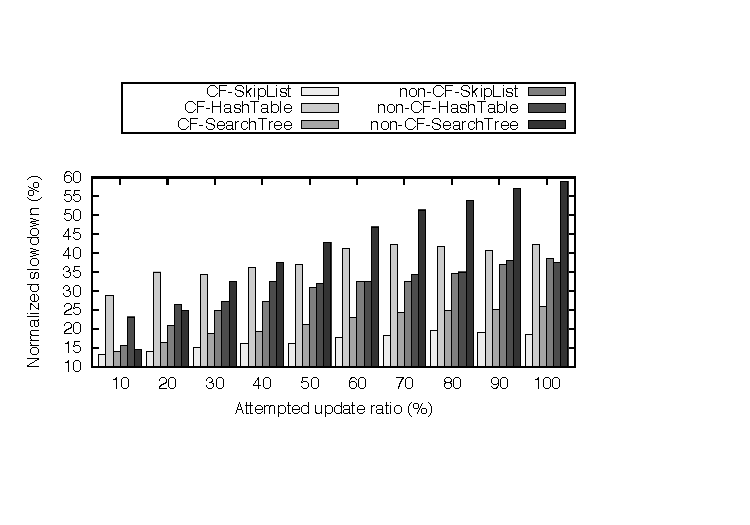
\includegraphics[scale=0.9,clip=true,viewport=10 50 280 230]{CF-general/experiments/pdf/updates}
\vspace{-1em}
\caption{\footnotesize{Tolerance to contention of Contention-Friendly (CF) and non-CF data structures (performance slowdown with respect to 0\% updates)\label{fig:updates}}}
\end{floatingfigure}
%
Interestingly, the slowdown of the CF hash table is higher than the one of the non-CF hash table at low 
levels of contention but becomes similar at high contention levels. 
As shown later, our CF hash table is actually very efficient on read-only workload whereas the ConcurrentHashMap relies on lock-stripes whose segments have to be loaded even on read-only workloads. 
This explains why CF performance drops as soon as contention appears, however, the CF hash table tolerates the contention increase as the slowdown remains almost constant, as opposed to the non-CF hash table.
We played with the number of segments and we observed better scalability with more segments but lower read-only overhead with a single one. We chose 64 segments which makes threads fetch multiple segments from memory before finding them in their cache. Another advantage of using  the CF hash table is not having to worry about such segments.

Figure~\ref{fig:perf} compares the performance of state-of-the-art data structures against performance of our CF data structures with $2^{14}$ (left) and $2^{16}$ elements (right) and on a read-only workload (top) and workloads comprising up to 30\% updates (bottom). While all data structures scale well with the number of threads, the state-of-the-art data structures are slower than their contention-friendly counterparts in all the various settings. In particular, the CF hash table, skip list, search tree are respectively up to $1.2\times$, $1.3\times$, $2.2\times$ faster than their non-CF counterparts.

Finally Appendix~\ref{sec:tm} shows that our adaptation of these data structures to three transactional memory algorithms allows a performance benefit of $1.5\times$ on average.

\begin{figure}
\begin{center}
\subfigure[$2^{14}$ elements\label{fig:214}]{\includegraphics[scale=0.45,clip=true,viewport=55 60 555 800]{CF-general/experiments/pdf/raw-perf-16384-60}}\hspace{0.5em}
%\caption{Performance of the Contention-Friendly (CF) and non-CF data structures with $2^{14}$ elements\label{fig:perf}}

\end{center}
\end{figure}
\begin{figure}
\begin{center}

\subfigure[$2^{16}$ elements\label{fig:216}]{\includegraphics[scale=0.45,clip=true,viewport=97 60 555 800]{CF-general/experiments/pdf/raw-perf-65536-60}}
%\caption{Performance of the Contention-Friendly (CF) and non-CF data structures with $2^{16}$ elements\label{fig:perf}}
\caption{Performance of the Contention-Friendly (CF) and non-CF data structures\label{fig:perf}}
\end{center}
\end{figure}



%\begin{figure}
%\begin{center}
%\includegraphics[scale=0.38]{experiments/pdf/raw-perf-16384-60}
%\caption{Performance of the Contention-Friendly (CF) and non-CF data structures with $2^{14}$ elements\label{fig:perf}}
%\end{center}
%\end{figure}
%
%\begin{figure}
%\begin{center}
%\includegraphics[scale=0.38]{experiments/pdf/raw-perf-65536-60}
%\caption{Performance of the Contention-Friendly (CF) and non-CF data structures with $2^{16}$ elements\label{fig:perf}}
%\end{center}
%\end{figure}


\section{Conclusion}\label{sec:conclusion}

Multicore programming brings new challenges, like contention, that programmers have to anticipate
when developing novel applications.
Programmers must now give up concentrating on the big-oh complexity and should
rather think in terms of contention overhead.
We explored the methodology of designing contention-friendly data structures, keeping in mind that contention will be a predominant cause of performance loss in tomorrow's architectures.
This simple methodology led to a novel Java package of concurrent data structures more efficient than the best implementations we could find. We plan to extend it with additional contention-friendly data structures.
%\vincent{Although transactions let the programmer take a pessimistic/sequential program as it is and make it concurrent, 
%the code requires to be significantly changed to be efficient.}

%\section*{Source Code}
%\sloppy{The Java code of the speculation-friendly library at \href{http://lpd.epfl.ch/gramoli/php/synchrobench.php}{http://lpd.epfl.ch/gramoli/php/synchrobench.php}.}
%
%\section*{Acknowledgements}
%The research leading to these results has received funding from the European Union Seventh Framework Programme (FP7/2007-2013) under grant agreement number 238639, ITN project TransForm, and grant agreement number 248465, the S(o)OS project.

% \newpage
% 
% \bibliographystyle{abbrv}
% \bibliography{bib}
% 
% \newpage
% 
% \begin{appendix}
% 
% % \section{Transactional Memory running CF skip list and CF binary search trees}\label{sec:tm}
% % \begin{figure*}
% % \begin{center}
% % 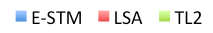
\includegraphics[scale=0.5]{./fig/legend-stms}\\
% % \subfigure[CF-SkipList vs. Pugh Skip List]{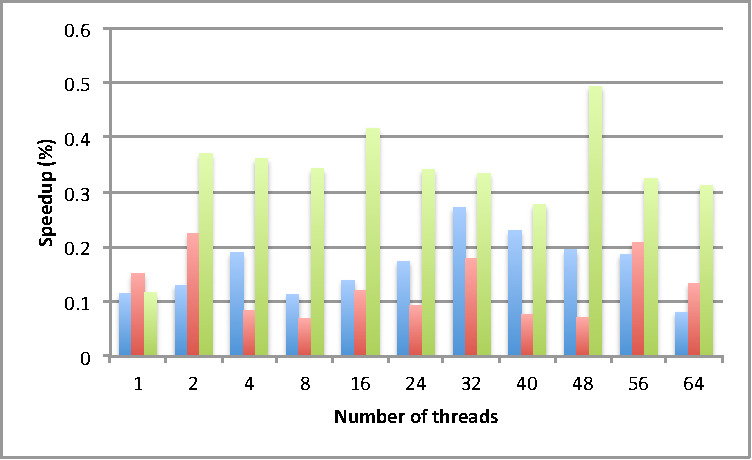
\includegraphics[scale=0.6]{./fig/skiplist-speedup}}
% % \subfigure[CF-Tree vs. RB-Tree]{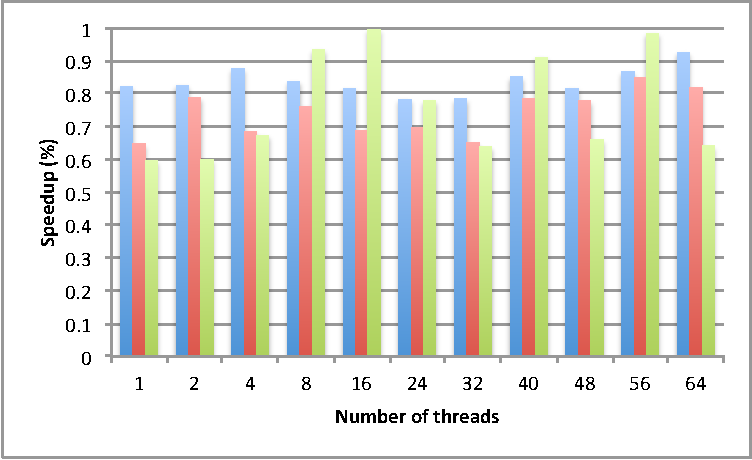
\includegraphics[scale=0.6]{./fig/tree-speedup}}
% % \caption{STM Speedup when using CF data structures instead of their existing counterparts on the Niagara 2 machine\label{fig:niagara2}}
% % \end{center}
% % \end{figure*}
% % 
% % \input alg/general3-1.tex
% 
% \input{appendix.tex}
% 
% \end{appendix}

%\section{Curves}
%
%\begin{figure*}
%\begin{center}
%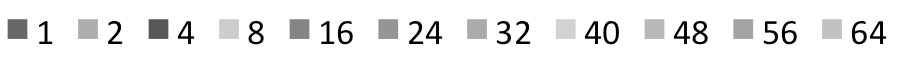
\includegraphics[scale=0.3]{./fig/legend-threadnum}
%\subfigure[$2^{12}$ elements, 0\% update]{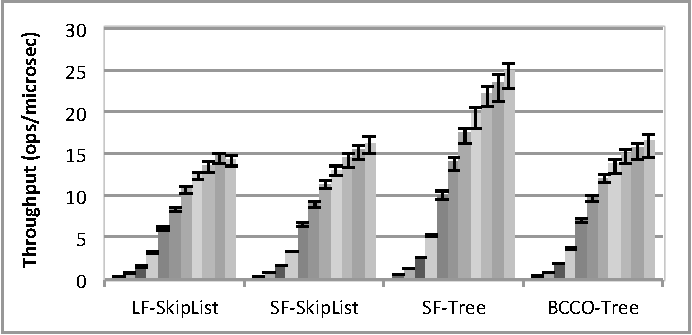
\includegraphics[scale=0.7]{./fig/nostms-logds-i4096-w0-bw.pdf}}
%\subfigure[$2^{12}$ elements, 10\% update]{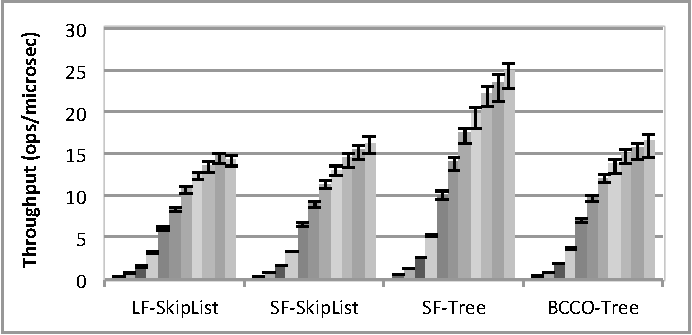
\includegraphics[scale=0.7]{./fig/nostms-logds-i4096-w0-bw.pdf}}
%\subfigure[$2^{12}$ elements, 20\% update]{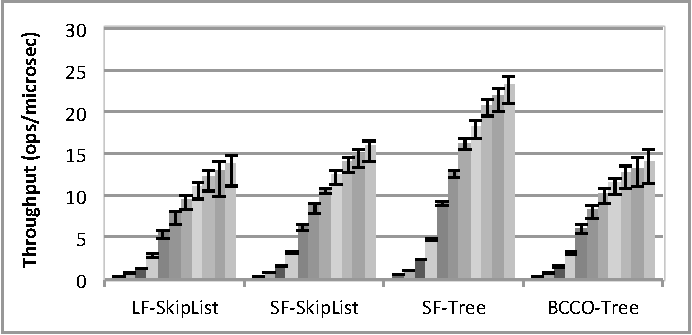
\includegraphics[scale=0.7]{./fig/nostms-logds-i4096-w10-bw.pdf}}
%\caption{Data structure (with logarithmic complexity) from the Niagara 2 machine\label{fig:niagara2}}
%\end{center}
%\end{figure*}

%\begin{figure*}
%\begin{center}
%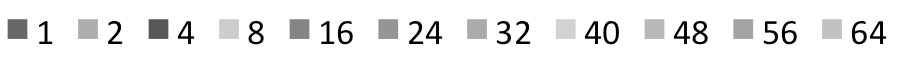
\includegraphics[scale=0.3]{./fig/legend-threadnum}
%\subfigure[$2^{14}$ elements, 0\% update]{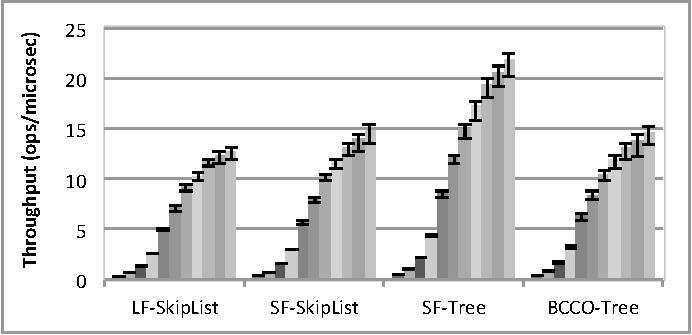
\includegraphics[scale=0.7]{./fig/nostms-logds-i16384-w0-bw.pdf}}
%\subfigure[$2^{16}$ elements, 0\% update]{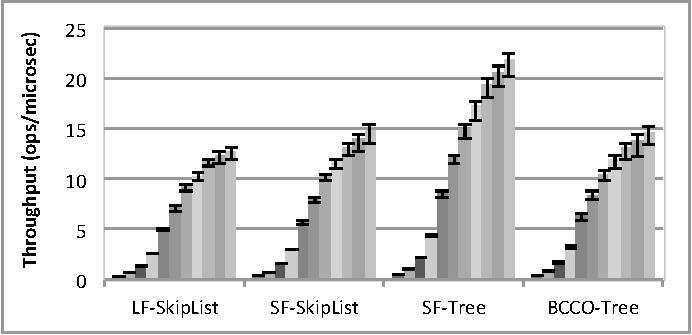
\includegraphics[scale=0.7]{./fig/nostms-logds-i16384-w0-bw.pdf}}
%\subfigure[$2^{14}$ elements, 10\% update]{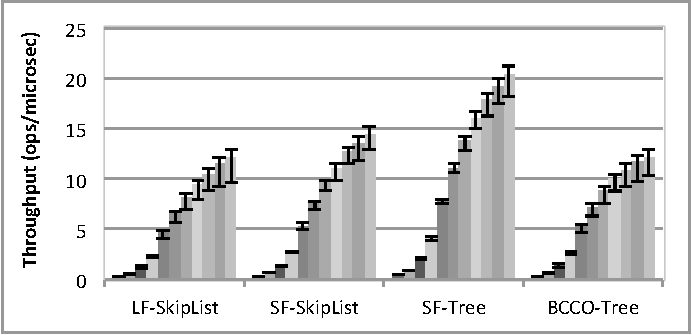
\includegraphics[scale=0.7]{./fig/nostms-logds-i16384-w10-bw.pdf}}
%\subfigure[$2^{16}$ elements, 10\% update]{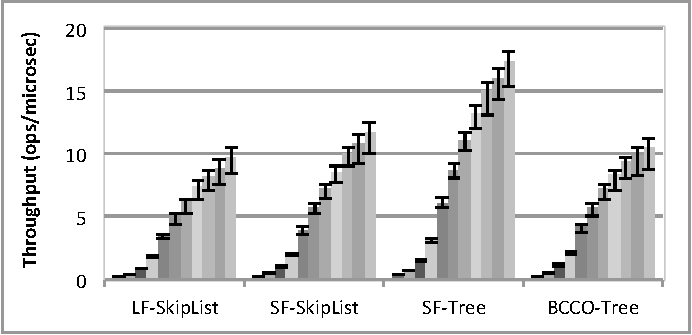
\includegraphics[scale=0.7]{./fig/nostms-logds-i65536-w10-bw.pdf}}
%\subfigure[$2^{14}$ elements, 20\% update]{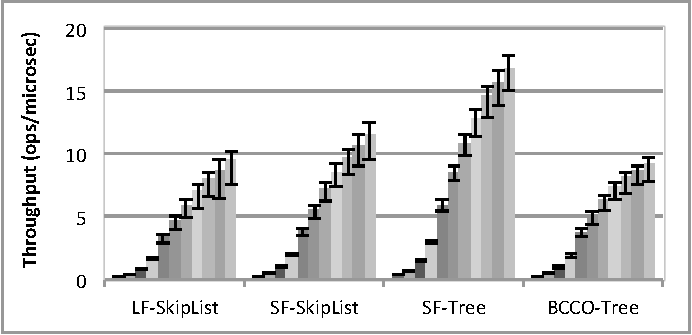
\includegraphics[scale=0.7]{./fig/nostms-logds-i65536-w20-bw.pdf}}
%\subfigure[$2^{16}$ elements, 20\% update]{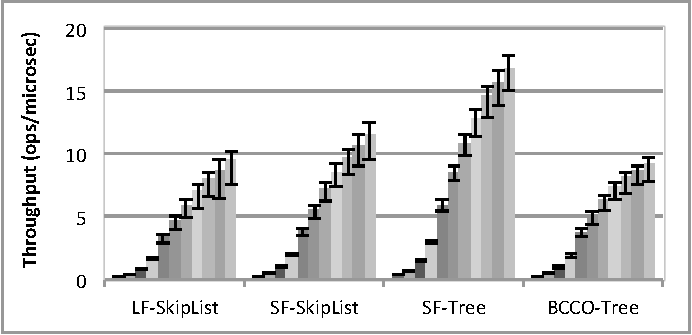
\includegraphics[scale=0.7]{./fig/nostms-logds-i65536-w20-bw.pdf}}
%\caption{Data structure (with logarithmic complexity) from the Niagara 2 machine\label{fig:niagara2}}
%\end{center}
%\end{figure*}


% Figure~\label{fig:niagara2} depicts the throughput performance obtained on the logarithmic data structures.
% 
% 
% \begin{figure*}
% \begin{center}
% 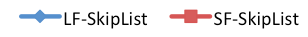
\includegraphics[scale=0.4]{./fig/legend-skiplist}\\
% \subfigure[$2^{12}$ elements, 0\% update]{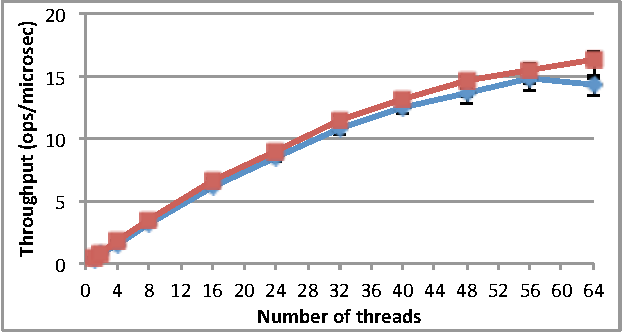
\includegraphics[scale=0.7]{./fig/nostms-sl-i4096-w0-bw.pdf}}\\
% \subfigure[$2^{12}$ elements, 10\% update]{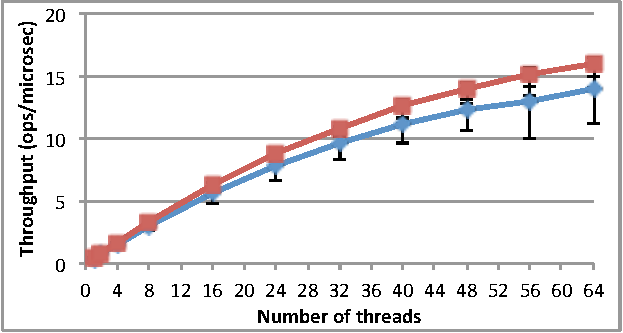
\includegraphics[scale=0.7]{./fig/nostms-sl-i4096-w10-bw.pdf}}\\
% \subfigure[$2^{12}$ elements, 20\% update]{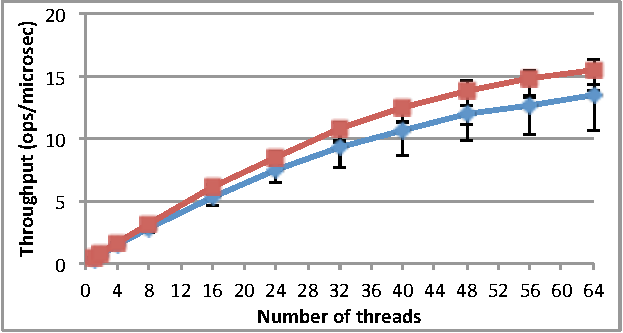
\includegraphics[scale=0.7]{./fig/nostms-sl-i4096-w20-bw.pdf}}
% \caption{Skip list results from the Niagara 2 machine\label{fig:niagara2}}
% \end{center}
% \end{figure*}
% 
% \begin{figure*}
% \begin{center}
% 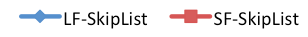
\includegraphics[scale=0.4]{./fig/legend-skiplist}\\
% \subfigure[$2^{14}$ elements, 0\% update]{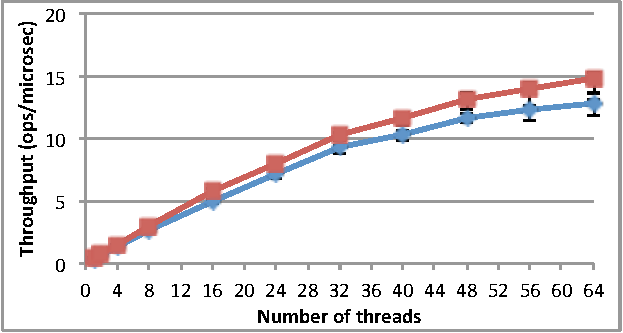
\includegraphics[scale=0.7]{./fig/nostms-sl-i16384-w0-bw.pdf}}
% \subfigure[$2^{16}$ elements, 0\% update]{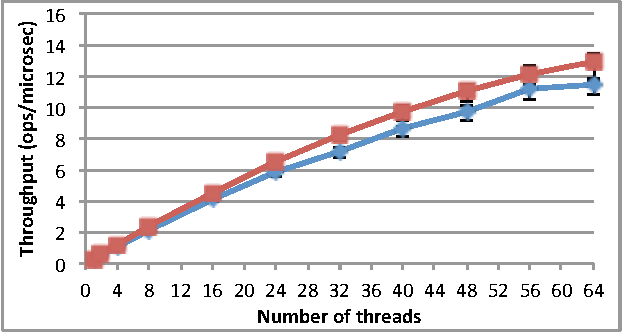
\includegraphics[scale=0.7]{./fig/nostms-sl-i65536-w0-bw.pdf}}
% \subfigure[$2^{14}$ elements, 10\% update]{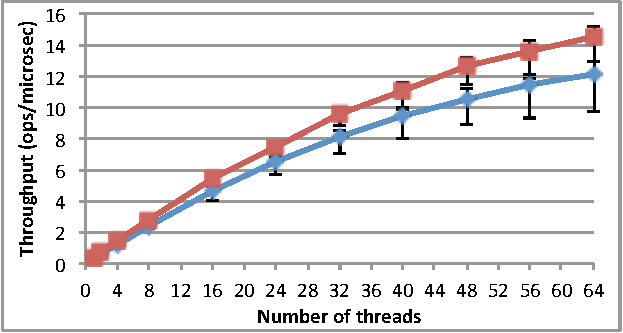
\includegraphics[scale=0.7]{./fig/nostms-sl-i16384-w10-bw.pdf}}
% \subfigure[$2^{16}$ elements, 10\% update]{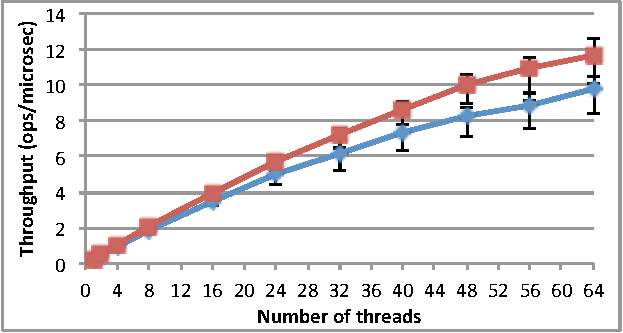
\includegraphics[scale=0.7]{./fig/nostms-sl-i65536-w10-bw.pdf}}
% \subfigure[$2^{14}$ elements, 20\% update]{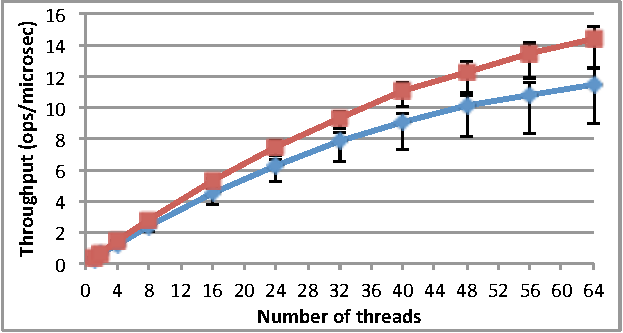
\includegraphics[scale=0.7]{./fig/nostms-sl-i16384-w20-bw.pdf}}
% \subfigure[$2^{16}$ elements, 20\% update]{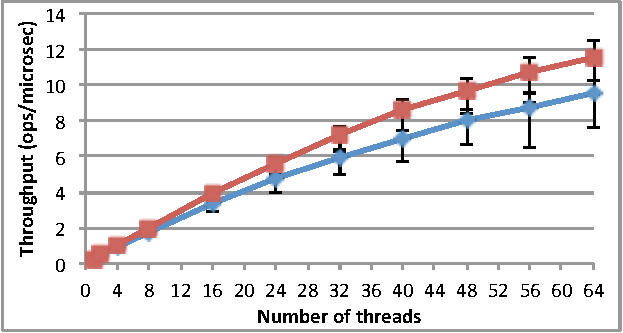
\includegraphics[scale=0.7]{./fig/nostms-sl-i65536-w20-bw.pdf}}
% \caption{Skip list results from the Niagara 2 machine\label{fig:niagara2}}
% \end{center}
% \end{figure*}
% 
% 
% \begin{figure*}
% \begin{center}
% 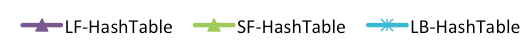
\includegraphics[scale=0.4]{./fig/legend-hashtable-2}\\
% \subfigure[$2^{12}$ elements, 0\% update]{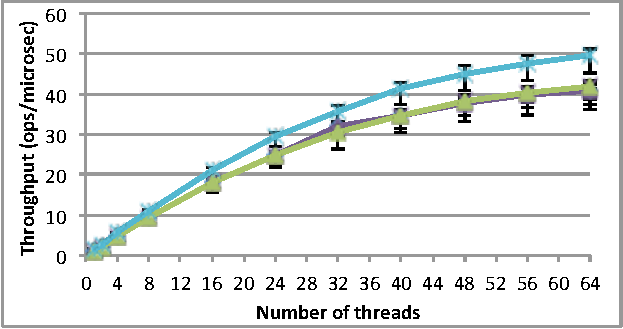
\includegraphics[scale=0.7]{./fig/nostms-ht2-i4096-w0-bw.pdf}}\\
% \subfigure[$2^{12}$ elements, 10\% update]{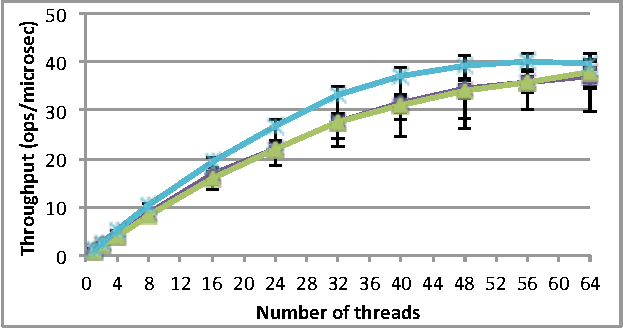
\includegraphics[scale=0.7]{./fig/nostms-ht2-i4096-w10-bw.pdf}}\\
% \subfigure[$2^{12}$ elements, 20\% update]{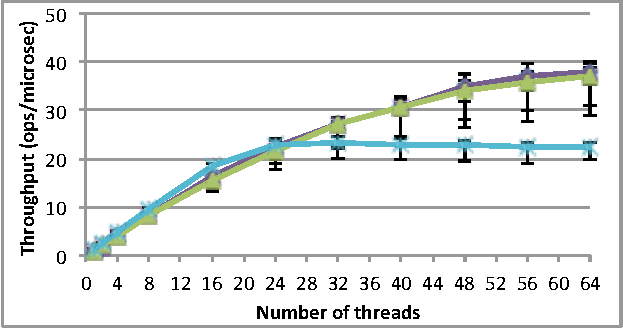
\includegraphics[scale=0.7]{./fig/nostms-ht2-i4096-w20-bw.pdf}}
% \caption{Hash table results from the Niagara 2 machine\label{fig:niagara2}}
% \end{center}
% \end{figure*}
% 
% 
% \begin{figure*}
% \begin{center}
% 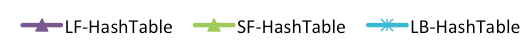
\includegraphics[scale=0.4]{./fig/legend-hashtable-2}\\
% \subfigure[$2^{14}$ elements, 0\% update]{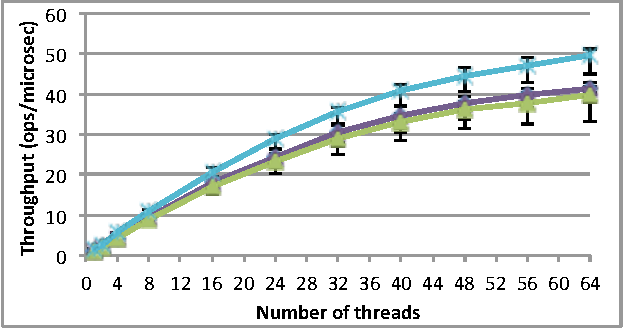
\includegraphics[scale=0.7]{./fig/nostms-ht2-i16384-w0-bw.pdf}}
% \subfigure[$2^{16}$ elements, 0\% update]{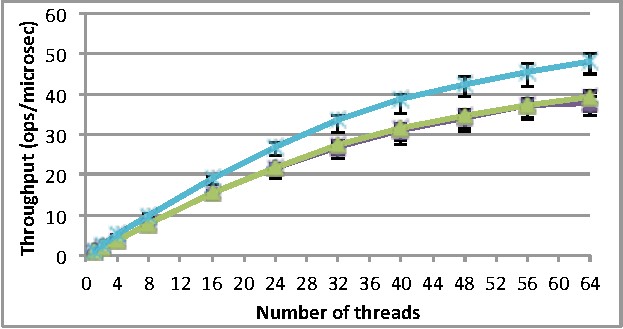
\includegraphics[scale=0.7]{./fig/nostms-ht2-i65536-w0-bw.pdf}}
% \subfigure[$2^{14}$ elements, 10\% update]{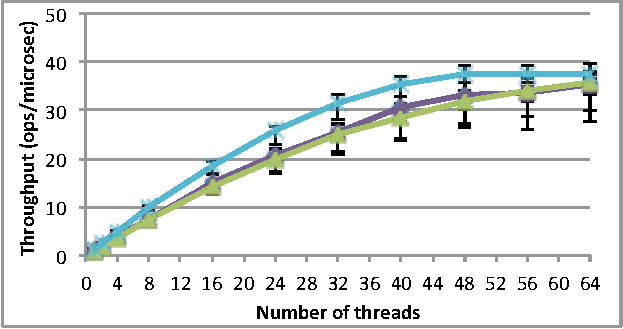
\includegraphics[scale=0.7]{./fig/nostms-ht2-i16384-w10-bw.pdf}}
% \subfigure[$2^{16}$ elements, 10\% update]{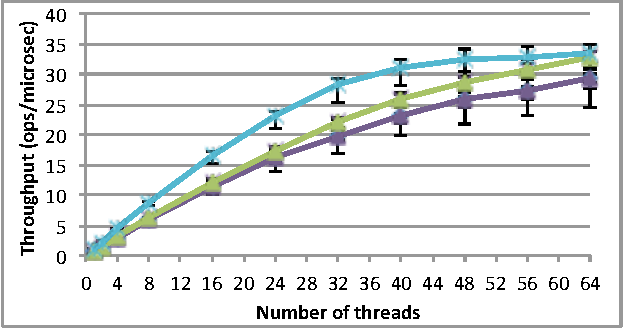
\includegraphics[scale=0.7]{./fig/nostms-ht2-i65536-w10-bw.pdf}}
% \subfigure[$2^{14}$ elements, 20\% update]{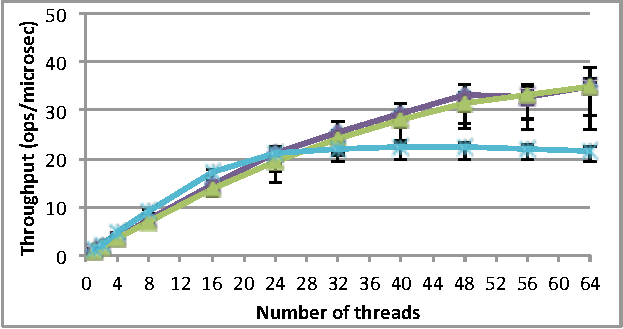
\includegraphics[scale=0.7]{./fig/nostms-ht2-i16384-w20-bw.pdf}}
% \subfigure[$2^{16}$ elements, 20\% update]{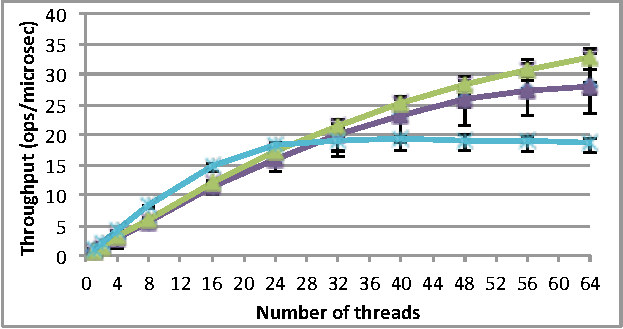
\includegraphics[scale=0.7]{./fig/nostms-ht2-i65536-w20-bw.pdf}}
% \caption{Hash table results from the Niagara 2 machine\label{fig:niagara2}}
% \end{center}
% \end{figure*}
% 
% 
% \begin{figure*}
% \begin{center}
% 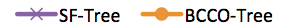
\includegraphics[scale=0.4]{./fig/legend-tree}\\
% \subfigure[$2^{12}$ elements, 0\% update]{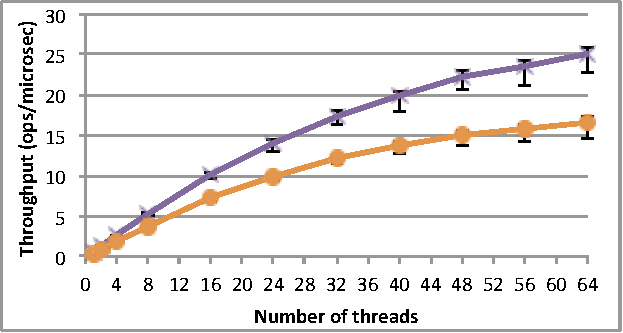
\includegraphics[scale=0.7]{./fig/nostms-tree-i4096-w0-bw.pdf}}\\
% \subfigure[$2^{12}$ elements, 0\% update]{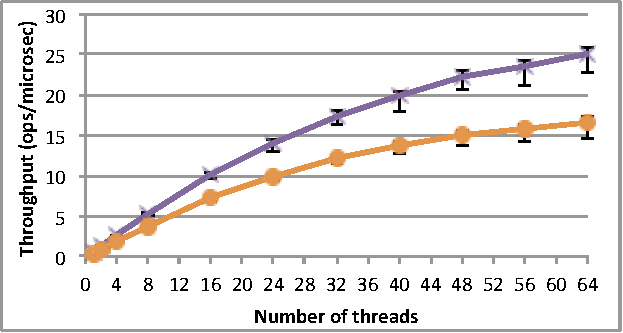
\includegraphics[scale=0.7]{./fig/nostms-tree-i4096-w0-bw.pdf}}\\
% \subfigure[$2^{12}$ elements, 10\% update]{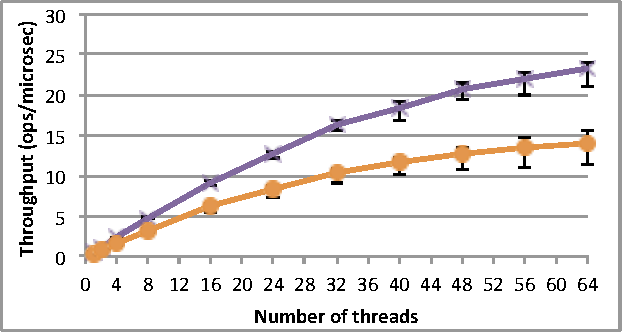
\includegraphics[scale=0.7]{./fig/nostms-tree-i4096-w10-bw.pdf}}
% \caption{Binary tree results from the Niagara 2 machine\label{fig:niagara2}}
% \end{center}
% \end{figure*}
% 
% 
% \begin{figure*}
% \begin{center}
% 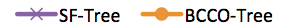
\includegraphics[scale=0.4]{./fig/legend-tree}\\
% \subfigure[$2^{14}$ elements, 0\% update]{\includegraphics[scale=0.7]{./fig/nostms-tree-i16384-w0-bw.pdf}}
% \subfigure[$2^{16}$ elements, 0\% update]{\includegraphics[scale=0.7]{./fig/nostms-tree-i65536-w0-bw.pdf}}
% \subfigure[$2^{14}$ elements, 10\% update]{\includegraphics[scale=0.7]{./fig/nostms-tree-i16384-w10-bw.pdf}}
% \subfigure[$2^{16}$ elements, 10\% update]{\includegraphics[scale=0.7]{./fig/nostms-tree-i65536-w10-bw.pdf}}
% \subfigure[$2^{14}$ elements, 20\% update]{\includegraphics[scale=0.7]{./fig/nostms-tree-i16384-w20-bw.pdf}}
% \subfigure[$2^{16}$ elements, 20\% update]{\includegraphics[scale=0.7]{./fig/nostms-tree-i65536-w20-bw.pdf}}
% \caption{Binary tree results from the Niagara 2 machine\label{fig:niagara2}}
% \end{center}
% \end{figure*}
% 
% 
% \begin{figure*}
% \begin{center}
% \includegraphics[scale=0.6]{./fig/legend-restructuring}\\
% \includegraphics[scale=0.7]{./fig/restructuring.pdf}
% \caption{Amount of restructuring observed on the Niagara 2 machine\label{fig:niagara2}}
% \end{center}
% \end{figure*}




% \end{document}



\section{Transactional Contention-Friendly Algorithms}\label{sec:tm} 


The concept of splitting the abstract operation and the structural modification to create contention friendly data structures
does not only apply to lock based or lock-free implementations.
It can also be applied to data structures implementations using transactional memory.
Our previous work has studied this problem when specifically looking at trees \cite{CGR12}.

%Figure \ref{fig:niagara2} shows the speedup of the contention friendly algorithms in transactional memory as compared
%to a red black tree and the Pugh Skip List which were converted from their sequential counterparts by placing their operations within transactions.
%In order to perform these tests we used the bytecode instrumentation 
%framework Deuce~\cite{KSF10}. Although this framework adds a significant overhead to the execution time, it greatly 
%simplifies the usage of various transactional memory algorithm. We have run the tests using the TM systems 
%TL2~\cite{DSS06}, LSA~\cite{RFF06}, and ${\mathcal E}$-STM~\cite{FGG09} illustrating the 
%portability of contention friendly data structures to TM systems satisfying the standard TM interface~\cite{abi}.
We now present the experimental results with three existing transactional memory implementations:
${\mathcal E}$-STM~\cite{FGG09}, LSA~\cite{RFF06} and TL2~\cite{DSS06} using the Deuce Java bytecode instrumentation framework~\cite{KSF10}.
The experimental settings are the same as for other experiments, except that we evaluate the red-black tree (non-CF tree) and the Pugh skip list (non-CF skip list) to compare our CF tree and CF skip list against on $2^{12}$ elements with 5\% effective updates.
Figure~\ref{sfig:tm-sl} and Figure~\ref{sfig:tm-rt}  depict the speedup of using the CF skip list over using the non-CF skip list (resp. CF tree over using the non-CF tree)
for each of the considered transactional memory implementations.
Using transaction-based CF data structures as opposed to default ones clearly speeds up the performance of all transactional memories. The benefit of turning to CF is more important when using trees, which confirms our previous results obtained with our lock-based implementations. In particular, the average speedup for all transactional memories and data structures is of 50\%.
Interestingly, the speedup of using transaction-based CF does not scale much with the number of threads, probably because the overhead induced by transactional memory and Deuce is too heavy for the contention rise to be visible.

When using transactional memory the benefit of these contention friendly algorithms is apparent just
by the fact that abstract operation transactions will have smaller read and write sets causing less contention
on the data structure and making the operations less likely to abort.
Also structural modifications are each broken into a single transaction causing less contention then they would
be if they were include in a single large transaction.

The abstract operations for the tree are very simple, traversals are done in the same way they would be in a
sequential algorithm except transactional reads are used.
Each physical removal and rotation is performed as a single transaction by the structural adaptation.

In the lock based version of the skip list locks are only used when traversing the bottom level of
the structure.
Each of the index levels are accessed and modified using only regular read/write operations.
This can be applied to the transaction version of the skip list as well.
Abstract operation traversals as well as structural modifications to the index level are done outside of transactions.
Once an abstract operation traversal has reached the bottom list level a transaction is started, if it arrived on
a physically removed node then the operation travels backwards in the list until is reaches a node still in the structure
at which point the traversal continues as it would in a sequential list algorithm.
Physical removals are done as single transactions by the structural adaptation.

The transactional hash table is very similar to the to the lock-free contention friendly version.
Each abstract operation is contained in a single transaction where the $\lit{compare\&swap}$
operations from the lock-free version are replaced by reads and writes.
During the rehash operation each bucket rehash is done as a single transaction.



\begin{figure*}
\begin{center}
%\includegraphics[scale=0.5]{./fig/legend-stms}\\
\subfigure[CF-SkipList vs. Pugh Skip List\label{sfig:tm-sl}]{\includegraphics[scale=0.85,clip=true,viewport=10 50 280 200]{CF-general/experiments/pdf/tm-skiplist}}
\subfigure[CF-Tree vs. RB-Tree\label{sfig:tm-rt}]{\includegraphics[scale=0.85,clip=true,viewport=10 0 280 200]{CF-general/experiments/pdf/tm-tree}}
\caption{STM Speedup when using CF data structures instead of their existing counterparts on the Niagara 2 machine\label{fig:niagara2}}
\end{center}
\end{figure*}


\section{Pseudo-code and Description}\label{app:pseudocode}

% \remove {
% 
% \subsection{Linked List}
% 
% \input alg/list_op.tex
% 
% \subsubsection{Non-maintenance Operations}
% The code for these operations is found in figure \ref{alg:list_op}.
% 
% The list nodes are standard doubly linked linked list nodes.
% To access the list there is a pointer $\ms{first}$ to the first node in the list.
% To simplify the algorithm the first node in the list is never removed and has key $\neg \inf$.
% 
% The traversal is very similar to the standard list traversal algorithm with one exception.
% When a traversal notices that is has reached a node that has been physically removed from the 
% structure (has $\ms{removed}$ flag set to $\lit{true}$)
% it travels backwards in the list (using the $\ms{prev}$ pointer) until it reaches a node that is 
% not removed.
% This is done to ensure that the traversal never passes the node it is searching for.
% 
% When adding an item to the list, the node that will be the node just before the new node is locked and the
% new node is inserted.
% 
% \input alg/list_maint.tex
% 
% \subsubsection{Maintenance Operations}
% The code for these operations is found in figure \ref{alg:list_maint}.
% Only maintenance needed for the list is performing physical removal.
% 
% To preform the removal, first the node to be removed and the node before it in the list is locked, then
% the $\ms{deleted}$ flag is check and the node is removed by changing the previous node's
% next pointer point to the next node and the previous pointer of this node is updated.
% Finally the node's removed flag is set to $\lit{true}$ and the nodes are unlocked.
% 
% }

All three data structures share the general structural adaptation code shown in Algorithm~\ref{alg:state-and-maintenance}.

In the normal case the structural adaptation thread works by performing the
$\ms{background-struct-adaptation}$ operation constantly traversing the data structure
by calling the $\ms{restructuring}$ procedure.
Each iteration of this procedure traverses the entire data structure where at each node it might perform some sort of restructuring or a removal.
For some data structures after a complete traversal of the structure is done, some restructuring of the entire structure might be needed,
this includes the rehash operation of a hash table or the changing of levels of nodes in the skip list.

For backwards compatibility the structural adaptation can also be distributed among the program threads by calling the 
$\ms{distributed-struct-adaptation}$ operation.
In this case each $\ms{insert/delete}$ operation will toss a coin, if the value of this coin is greater then some threshold value
the thread will then acquire a global structural adaptation lock, and call the $\ms{restructuring}$ procedure before finally
releasing the lock, and continuing with its abstract operation.


\subsection{Tree and Skip List}

\paragraph{Skip List}
As with existing skip list algorithms the structure is made up of many levels of linked lists.

The bottom level of is made up of a doubly linked list of nodes.
Each node has a $\ms{prev}$ and $\ms{next}$ pointer, as well as pointer to its key $\ms{k}$,
an integer $\ms{level}$ indicating the number of levels of linked lists this node has,
the $\ms{rem}$ and $\ms{del}$ flags, and a lock.

The upper levels are made up of singly linked lists of IndexItems.
Each of these items has a $\ms{next}$ pointer, pointing to the next item in the linked list.
A $\ms{down}$ pointer, pointing to the linked list of IndexItems one level below (the bottom level
of IndexItems have $\bot$ for their $\ms{down}$ pointers).
And a $\ms{node}$ pointer that points to the corresponding node in the Speculation Friendly Skip List.

A per structure array of pointers called $\ms{first}$ is also kept that points to the first element of each level
of the skip list.
The pointer $\ms{top}$ points to the first element of the highest index of the list, all traversals
start from this pointer.

\paragraph{Tree}
The tree is made up of nodes with each node having left and right child
pointers $\ms{l}$ and $\ms{r}$, as well as a pointer to its key $\ms{k}$,
integers indicating the estimated local height
of this node and its children $\ms{left-h}$, $\ms{right-h}$, and $\ms{local-h}$,
the $\ms{rem}$ and $\ms{del}$ flags, and a lock.

In addition there is a single pointer $\ms{root}$ that points to the root node of
the tree.

\subsubsection{Skip List Structural Adaptation}

\input CF-general/alg/skipList_maint.tex

The code for the skip list structural adaptation operations is found in Algorithm~\ref{alg:skipList_maint}.

The $\ms{restructure-node}$ procedure takes care of removing marked deleted nodes.
For each node it checks if it has both a level of $0$ and $\ms{del}$ set to $\lit{true}$
then tries to remove the node by calling the $\ms{remove-node}$ procedure.
This procedure locks both the node to be removed and the node previous to it in the list in order
to not conflict with concurrent $\ms{insert}$ and $\ms{delete}$ operations.
The node is then simply removed by changing the previous node's pointer to skip the node.
Finally the $\ms{rem}$ flag is set to true and the locks are released.

The $\ms{restructure-structure}$ procedure raises and lowers the levels of the nodes in order
to keep the logarithmic traversal cost of the abstract operations.
This is done by calling the $\ms{raise-node-level}$ procedure on the bottom level of the
skip list and the $\ms{raise-index-level}$ on higher levels.
The code for the procedures is practically the same, just $\ms{raise-node-level}$ is performed
on nodes while $\ms{raise-index-level}$ is performed on index levels as such only the 
$\ms{raise-index-level}$ pseudo code is displayed here.
The procedures work by simply traversing the entire level $\ms{i}$ that they are called on
if they encounter $3$ or more nodes all with height $\ms{i}$ then the middle of these
nodes is raised to height $\ms{i+1}$.
This is performed on each index level starting from the bottom until there are less than $2$
nodes on a level.

Due to nodes being removed from the skip list it might be necessary to decrease
the number of index levels in the structure.
If the $log$ of the number of nodes in the structure is less then the height of
the structure then the bottom index level is removed.
This is done by the $\ms{lower-index-level}$ procedure which simply traverses
the second from bottom index level and sets each index item's $\ms{down}$ pointer to $\bot$.
Finally the index of the $\ms{first}$ array must be updated to take account
the removal of the bottom index level.

\input CF-general/alg/tree_maint.tex

\subsubsection{Tree Structural Adaptation} \label{sec:treemaint}
The code for these operations is found in Algorithm~\ref{alg:tree_maint}.

The $\ms{restructure-node}$ procedure takes care of removing marked deleted nodes as well as
performing rotations and propagating balance information upwards in the tree.

Like in the skip list only certain nodes are removed.
These are the nodes that have $1$ or $0$ children and are a majority of the nodes in the tree.
This avoids expensive removal operations that require finding
and moving a successor node.

In order to do a removal first the parent and the node to be removed are locked(in order to
prevent conflicts with concurrent $\ms{insert}$ and $\ms{delete}$ operations) and the
$\ms{del}$ flag of the node is checked.
The node to be removed has its $\ms{left}$ and $\ms{right}$ child pointers changed so that they point to the parent.
This is done to ensure a concurrent operation preempted on this node can still proceed.
Next the appropriate parent's child pointer is changed to point to the non-null child of the node to be removed
(if any).
Finally the $\ms{rem}$ flag is set to $\ms{true}$.

% 
% \begin{figure*}
% 	%\vspace{-1em}
% 	\begin{center}
% 	\subfigure[Initial tree\label{sfig:tree1}]{\includegraphics[scale=0.4]{fig/tree1b}}\hspace{4em}
% 	\subfigure[Result of usual right rotation\label{sfig:tree2}]{\includegraphics[scale=0.4]{fig/tree2b}}\hspace{4em}
% 	\subfigure[Result of new right rotation\label{sfig:tree3}]{\includegraphics[scale=0.4]{fig/tree3b}}
% 	\caption{The classical rotation modifies node $j$ in the tree and forces a concurrent traversal at this node to backtrack. 
% 	The new rotation left $j$ unmodified, adds $j'$ and postpones the 
% 	physical deletion of $j$.\label{fig:rotation}}
% 	\end{center}
% 	%\vspace{-1em}
% \end{figure*}


The structural adaptation is also responsible for keeping the tree well balanced.
This is done by doing local rotations.
Deciding to do a rotation is based on a local estimated height values.
The height values are propagated from the leaves to the root by the $\ms{propagate}$ procedure.
This procedure is executed per node and simply reads the $\ms{l-height}$ values of its left
and right children, before updating its local values and setting its local $\ms{l-height}$ value
to $1$ greater then the maximum height of its children.
If the absolute value of a nodes left and right heights is at least two
then an appropriate rotation is performed.
Double rotations are performed as two separate single rotations.

In a traditional rotation operation one node is always rotated downwards.
If a concurrent traversal operation is preempted on this node then either it might have to abort
or rollback in order to ensure it performs a valid traversal or nodes must be locked/marked during traversal.

In order to avoid using locks and aborts/rollbacks, rotations are preformed differently then traditional rotations.
A diagram of the new rotation operation is shown in figure \ref{sfig:tree3}.
Before performing the rotation the parent node and the node $\ms{n}$ that will be rotated are locked in order to
prevent conflicts with concurrent $\ms{insert}$ and $\ms{delete}$ operations.
Instead of actually modifying $\ms{n}$, a new node $\ms{new}$ is created that takes $\ms{n}$'s place in the structure,
this node is set have the same values and pointers as $\ms{n}$ would if a rotation was performed as in
existing tree data structures.
After the rotation, the node $\ms{n}$ has its $\ms{rem}$ flag set (to $\lit{true}$ in the case of a right rotation
and $\lit{by-left-rot}$ in the case of a left rotation) and the locks are released.

The reason for not modifying $\ms{n}$ is so that concurrent traversals are not set off track.
If the node $\ms{n}$ is removed by a right (resp. left) rotation then its left (resp. right) child has a path to
all the nodes as it did before the rotation so a traversal preempted on this node can still traverse the tree safely.

\input CF-general/alg/general3-1.tex
\input CF-general/alg/general3-2.tex
\subsection{Abstract Operations}

The tree and skip list share code for the $\ms{contains}$, $\ms{insert}$, $\ms{delete}$ operations
displayed in Algorithm~\ref{alg:general_op-2}.
These operations might call one of more of the $get\_first$, $get\_next$, $validate$, $add$
procedures which each have specific code for the given data structure,
show in Algorithm~\ref{alg:tree_op} for the tree and Algorithm~\ref{alg:skipList_op}
for the skip list.
None of these additional procedures use locks or other synchronization methods.

\input CF-general/alg/skipList_op.tex
\input CF-general/alg/tree_op.tex

Each of the three abstract operations start by calling the $\ms{get\_first}$ procedure.
This operation returns the root of the tree or the first node of the top index level of the skip list.
The operations then traverse the structure using the $\ms{get\_next}$ procedure.
This procedure either returns the next node in the traversal or $\bot$ if the traversal is done.

The $\ms{get\_next}$ procedure traverses the tree by returning the right child if the node's key is lager then $k$
otherwise the left child is returned.
If the nodes key is equal to $\ms{k}$ and the node is not physically removed then $\bot$ is returned.
Since locks are not used during traversal the algorithm has to be aware of concurrent rotations.
This means returning the right child in case of being preempted on a node that was removed during a left rotation.
If the node was removed during a right rotation then the traversal can continue as normal unless it arrives at a
child pointer with value $\bot$, in this case it just returns the other child (which is guaranteed to not be $\bot$).

For the skip list the $\ms{get\_next}$ procedure traverses the structure just as it would in a sequential
algorithm, with the simple exception that is travels backwards in the list using the $\ms{prev}$ pointer
in the case of arriving at a node that has been physically removed.
If the nodes key is equal to $\ms{k}$ and the node is not physically removed or if the traversal
is at the bottom level and the next node has key greater then $\ms{k}$ then $\bot$ is returned.

Once $\bot$ is returned $\ms{insert}$ and $\ms{delete}$ operations protect the last node in the traversal by locking it (locking is not necessary for the $\ms{contains}$ operations as
it does not make modifications).
Due to concurrent operations this node may not longer be the end of the traversal, therefore the $\ms{validate}$ procedure is performed on this node
ensuring that the traversal has stopped at the correct location.
The validation checks to make sure that the node has not been physically removed and that no new node has been inserted directly after this node.

If the validation succeeds then the traversal is finished.
Otherwise the lock protecting the node
is released and the traversal continues.

Finally some additional code is executed depending on the operation.

In the case of a $\ms{contains}$ operation, the key and/or the deleted flag of the node is checked and a boolean is returned.

In the case of the $\ms{insert}$ operation, first the key of the node is checked, if it is equal to the key being search for then
the deleted flag of the node is checked (and possibly modified) and a boolean is returned.
Otherwise if the key is not equal to the one being searched for then the $\ms{add}$ operation is performed.
The code for the $\ms{add}$ operation simply allocates a new node and attaches
it to the data structure by modifying a pointer.

In the case of the $\ms{delete}$ operation the key of the node is checked, if it is equal to the key being search for then
the deleted flag of the node is checked (and possibly modified) and a boolean is returned.
Otherwise $\lit{false}$ is returned.
It should be noted that when these structures are used as maps the deleted flag can be replaced with a pointer to the
value object (from the key/map pair).
When this pointer is set to $\bot$ the node is considered as deleted.



\subsection{Hash Table}

The hash table is made up of two pointers to tables:
$\ms{table}$ and $\ms{new\_table}$.
The second is used during resize operations.
Each process also keeps local variable $\ms{l\_pointer}$ that points to a table.

Each table contains an array, with each location in the array containing a list of nodes.
Each location in the array is initialized to point to $\bot$.
The array also has a single special node associated with it called the $\ms{dummy}$ node which is used
during resizing.

\input CF-general/alg/hashTable_op.tex

\subsubsection{Abstract Operations}
The code for these operations is found in Algorithm~\ref{alg:hashTable_op}.
Each abstract operation starts by calculating the hash value of the key and then calling
the $\ms{get-first}$ procedure.
This procedure returns the first node in the table located at the bucket given by the hash value
or $\bot$ in the case that this bucket is empty.
The $\ms{get-first}$ procedure might encounter a dummy node, this means that there is a rehash operation
going on that has rehashed this bucket, but not yet finished rehashing the entire table.
In this case the local table pointer is updated and the bucket is read again.

Once a value is received from the $\ms{get-first}$ procedure the $\ms{contains}$ simply traverses
the list looking for a node with key $\ms{k}$.

The $\ms{insert}$ operation also traverses
the list looking for a node with key $\ms{k}$, if none is found then a new node is allocated and is
added to the beginning of the list by performing a $\lit{compare\&swap}$ on the bucket.
If the $\lit{compare\&swap}$ fails then the operation restarts.

If the $\ms{delete}$ operation locates a node $\ms{n}$ with key $\ms{k}$ in the list
then it creates a copy of the list from the first node in the list up to node $\ms{n}$ but not including $\ms{n}$.
The bucket is then set to first node of this list by performing a $\lit{compare\&swap}$.
If the $\lit{compare\&swap}$ fails then the operation restarts.


\input CF-general/alg/hashTable_maint.tex

\subsubsection{Structural Adaptations}
The code for these operations is found in Algorithm~\ref{alg:hashTable_maint}.
Local node restructuring is not necessary for the hash table.

The structure restructuring consists of two procedures.
The first is the $\ms{size}$ operation that simply traverses the structure
counting the number of nodes.
If the number of nodes has surpassed some threshold then a resize is necessary
and the $\ms{grow}$ procedure is called.
This procedure starts be creating a new table larger then the previous one
by a power of $2$.
It then goes through the old table rehashing one bucket at a time.
At each bucket in the old table it performs the $\ms{grow-level}$ procedure.
This procedure makes a copy of each node in the bucket, rehashing them and placing them
in their appropriate buckets in the new hash table.
The operation then replaces the list in the old table with its dummy node by performing a
$\lit{compare\&swap}$.
If the compare and swap fails then the operation is restarted for this level.
Once all levels have been rehashed the $table$ pointer is modified so that it points
to the new table.

\section{Correctness}\label{sec:proof}






Here we present a sketch of the proof that each data structure algorithm satisfies linearizability.

\subsection{Skip List}

Each of the $\ms{contains}$, $\ms{insert}$, and $\ms{delete}$ operations call the $\ms{validate}$ procedure.
The $\ms{validate}$ procedure may be called multiple times, but it must return $\lit{true}$ exactly once.
This is used as the linearizability point for the proof sketch.
Assume $\ms{k}$ the key provided as input to the abstract operation.

The result of the $\ms{contains}$, $\ms{insert}$, and $\ms{delete}$ operations depends on the existence of
a node with key $\ms{k}$
in the set described by the data structure.
At any single point in time there is exactly one valid location in the list where a node with key $\ms{k}$ can exist
(Note that a full proof would require to show this, for example by induction).
This location is the $\ms{next}$ pointer of the node in the list with the largest key smaller then $\ms{k}$.
For the purpose of this proof sketch we will use a node (call this node $\ms{corr}$) that is either the node in the list
with key $\ms{k}$ or if no node with key $\ms{k}$ exists the node whose $\ms{next}$ pointer would point to the node with key $\ms{k}$.

Any operation that modifies a node must lock the node before it performs any modification.
Given that the $\ms{validate}$ operation is called while a node is locked it only needs to be shown
that the when $\ms{validate}$ returns $\lit{true}$ the node locked is $\ms{corr}$.

The nodes in the list are sorted by their keys and the $\ms{prev}$ pointer is not modified when a node is removed
so any removed node will always have a path to a non-removed node with a smaller or equal key.
This means that there will always be a path from a node with key smaller then or equal to $\ms{k}$ to $\ms{corr}$.
Now since the $\ms{get-next}$ procedure will never traverse past a node that has key larger then $\ms{k}$ the operation it will always have
a path to $\ms{corr}$.
If a node that has been removed is reached during traversal the $\ms{prev}$ pointer is followed, otherwise the $\ms{next}$ pointer
is followed during traversal so $\ms{corr}$ will be reached eventually.

Before the $\ms{validate}$ operation returns $\lit{true}$ it first ensures that the locked node has either key $\ms{k}$ or the node pointed
to by the locked node's $\ms{next}$ pointer has a key larger then $\ms{k}$.
Second it ensures that the node is not removed ($\ms{rem}=\lit{false}$).
Therefore when $\ms{validate}$ returns $\lit{true}$, the locked node must be $\ms{corr}$.

\subsection{Tree}
The tree is a bit more complicated because traversals have to deal with
rotations as well as removals.
Like in the skip list the abstract operations can call the $\ms{validate}$ procedure multiple times, but it must return $\lit{true}$ exactly once.
This is used as the linearizability point for the proof sketch.
Assume $\ms{k}$ is the key provided as input to the abstract operation.

At any point in time there is exactly one valid location in the tree where a node with key $\ms{k}$ can exist.
This location is the left or right child pointer of a certain node.
This pointer points to the node with key $\ms{k}$ or to $\bot$ if no node with key $\ms{k}$ exists.
For the purpose of this proof sketch we will use a node (call this node $\ms{corr}$) that is either the node with
this pointer (if no node with key $\ms{k}$ exists) or the node with key $\ms{k}$ (is a node with key $\ms{k}$ does exist).

Before the $\ms{validate}$ operation returns $\lit{true}$ it first ensures that the locked node either has key $\ms{k}$ or
(if the locked node does not have key $\ms{k}$) the
child pointer from the locked node where $\ms{k}$ would exist is $\bot$.
Second it ensures that the locked node is not removed ($\ms{removed}=\lit{false}$).

Now to complete the sketch it is enough to show that the traversal never passes $\ms{corr}$.
Without rotations or removals this is simple.
With removals and rotations the idea is to show that a traversal that is preempted on a node modified by a removal or rotation
operation has a path to a node at a higher level in the tree so that the traversal still has a path to $\ms{corr}$.
For removals this is clear due to the fact a removed node has both its child pointers point to its parent during removal.
Rotations require a bit more detail.
In a traditional left/right rotation one node is rotated downward in the tree while either its left or
right child is rotated upwards.
For rotations in the contention friendly algorithm the child pointers of the node that
would normally be rotated downwards (call this node $\ms{n}$) are not modified at all.
Instead $\ms{n}$ is removed from the tree (as the previous parent of $\ms{n}$ now points to one of $\ms{n}$'s children)
and a new node is created taking $\ms{n}$'s place.
This new node is set up exactly how $\ms{n}$ would be after a traditional rotation.
Now since one of $\ms{n}$'s children was rotated upwards any concurrent traversal preempted on $\ms{n}$ will
still have a path to all the nodes it did before the rotation.

\subsection{HashTable}
The linearization of the hash table relies on two things, first that the $next$ pointer of a node is never modified
after it is set during creation, and second any successful modification to a bucket happens by performing a
single $\ms{compare\&swap}$ on the bucket's pointer.

The linearization point of the $\ms{contains}$ operation is when the $\ms{get-first}$ procedure reads the first element of the
bucket that is later returned.
Since the next pointer of nodes is never changed then when the operation traverses the list it observes a valid state of the list.
The same is true for $\ms{insert}$ and $\ms{delete}$ operations that complete without performing a $\ms{compare\&swap}$.

If a $\ms{compare\&swap}$ is required, then the lineraization point is when the $\ms{compare\&swap}$ returns successfully.
Given that the $\ms{compare\&swap}$ operations are only performed at the first element of the bucket, if the operation succeeds then
the lineraiztion is valid because
the list at the bucket has not changed since $\ms{get-first}$ procedure read it.





\section{Garbage Collection}
Nodes that are physically removed from the data structures must be garbage collected.
In the tree and skip list nodes are physically removed only by the structural adaptations.
This can happen during rotations of the tree, during the lowering of levels in the skip list,
or during the $\ms{remove}$ operation of either structure.
Nodes of the hash table are physically removed by the abstract $\ms{delete}$ operation or by the rehash structural adaptation operation.
Once a node is physically removed it will no longer be pointed to by the data structure meaning that no future operation
will traverse these nodes.

Concurrent traversal operations could be preempted on a removed node so the node cannot be freed immediately.
In languages with automatic garbage collection these nodes will be freed as soon as all preempted traversals continue past this node.
If automatic garbage collection is not available then some additional mechanisms can be used.
One possibility is to provide each thread with a local operation counter and a boolean indicating if the tread is currently performing
an abstract operation or not.
Then any physically removed node can be safely freed as long as each thread is either not performing an abstract operation or if it has increased its
counter since the node was removed.
Normally this should be done during the structural adaptation.

\section{Future Work}

\subsection{Lock-freedom}
The tree and skip list algorithms presented in this paper use locks.
By using locks they are susceptible to problems such as a thread crashing or being descheduled while holding a lock.
In order to avoid these problems, certain concurrent algorithms such as have been designed to be
lock-free such as \cite{Fra03}.
Lock-free algorithms are generally considered to be complex and difficult to program.
This paper focuses on the methodology of designing contention friendly data structures rather then
deep descriptions of the algorithms.
For this reason the algorithms are described using locks and a brief intuition on how to make
the algorithms lock free is given here.

Lock free algorithms often rely on atomic synchronization primitives such as $\lit{compare\&swap}$ in order to preform tasks without using locks.
Often a more complex task will require more then just a single atomic operation.
In this case one thread might be required to help another thread's operation so that it completes
without blocking other operations.

The $\ms{insert}$, $\ms{delete}$, $\ms{contains}$ operations of the contention friendly data structures are simple enough to only require
at most one $\lit{compare\&swap}$ operation to complete.
For an $\ms{insert}$ this might be performing a $\lit{compare\&swap}$ on a pointer and for a $\ms{delete}$ this might be
performing a $\lit{compare\&swap}$ on a flag.

The structural adaptation thread takes care of the more complex operations such as removals and
modifications to the structure, operations that might require more then just a single 
$\lit{compare\&swap}$.
Consider a $\ms{remove}$ operation, the structural adaptation thread will initiate the removal by performing a 
$\lit{compare\&swap}$
to flag the node letting other processes know that it will be removed.
The actual removal is then preformed which requires several more $\lit{compare\&swap}$s.
Before the removal is completed another thread might concurrently traverse the flagged node while searching for some key at a different location
in the structure.
Like in the lock based algorithms this is fine and the traversal can continue as normal.
On the other hand a concurrent traversal might need to perform its operation at the location of the node being removed,
for example it might need to insert a new node just after the node.
In this case the traversal will help the structural adaptation thread with the removal before completing its operation.

In the lock-free version of the concurrent friendly skip list the structural adaptation thread is in charge of removals and
raising and lowers of heights of nodes.
The raising and lowering of heights can be done just as in the lock based version since no synchronization is required.
The removal of nodes uses the same process as in~\cite{Fra03} except the structural adaptation thread will start the removal and
program threads will help as necessary.

In the tree removals as well as rotations are performed by the structural adaptation thread and might be helped by
program threads.
Each of these operations is started by the structural adaptation thread performing a 
$\lit{compare\&swap}$ to flag the node.
The only non-blocking implementation of a binary search tree that we know of is presented in~\cite{EFRB10}.
This tree is \emph{leaf-oriented} where keys are stored in leaf nodes.

Even though we do belive it would be possible to implemnt these lock-free algorithms we do expect them to be very complex
and would require more investigation.

\subsection{Structural Adaptation Throttling}
In the default version of these algorithms a separate structural adaptation thread is created that continually
traverses the tree performing structural modification as necessary.
In workloads with low update rates this constant traversal will not have any modification to perform,
wasting computation.
Even if there are extra unused cores this extra computation may be unwanted due to additional power
consumption.
Future work should include studying way to throttle the structural adaptation dynamically based on the workload.
This could mean putting the thread to sleep during periods of low update rate or even starting
and stopping the structural adaptation thread entirely.
In largely parallel workloads with high update rates it might even be beneficial
to have multiple structural adaptation threads that can be started and stopped at will.

\subsection{Distributed Structural Adaptation}\label{sec:disMaint}
Each structural adaption is a short local operation, yet each round of structural adaptation is done by a complete traversal
of the data structure.
Some might argue that if all the hardware of a system is already in use by program threads then why not break the structural adaptation
into smaller structural adaptations and distribute them over the abstract modifications.
The reason for not doing this is twofold.

Firstly even though each structural adaption is a very local operation, they use global information.
For example rotations in a tree need balance information that is propagated from the leaves.
Since only nodes with height $1$ are removed from the skip list the structural adaptation needs to know about the heights
of the other nodes before raising the level of a node in order to ensure that the structure does not become unbalanced.
Before resizing the hash table the structural adaptation should know approximately how many nodes are in the table.

Secondly the structural adaptations are in some cases more costly (in terms of computation, not contention) then in existing data structures.
For example a rotation requires allocating a new node, choosing the levels of nodes in the skip list
requires previously traversing the other nodes to know their height, and resizing the hash table first requires
counting the nodes.

Such algorithms with distributed structural adaptation might be possible, but have not been examined here, but could be
interesting to study in the future.
